\documentclass[]{article}
\usepackage{amsmath}
\usepackage[sorting=none]{biblatex}
\addbibresource[datatype=bibtex]{refs.bib}
\addbibresource[datatype=bibtex]{homodyne.bib}
\usepackage{csquotes}
\usepackage[]{subcaption}

\usepackage{hyperref}
\usepackage{graphicx}


\usepackage{xcolor}
\usepackage{soul}
\let\phi\varphi
\title{On the asymmetrical strong Local Oscillator approximation} %мб?
\author{MbI}
\begin{document}
\maketitle
\section{Abstract}
The statistical photon count distribution in homodyne measurement is well known. From the exact formulae, it is possible to obtain the so-called strong local oscillator approximation, which reveals some properties of the signal state. For this approximation to accurately describe a physical process, an appropriate positive-valued operator measure (POVM) must be constructed.

Our analysis focuses on the case of an unbalanced beam splitter and unequal non-unity quantum efficiency of the photodetectors, which we refer to as the asymmetrical case, in contrast to the traditionally studied symmetrical case of a balanced beam splitter and equal non-unity quantum efficiencies. We derive {the} approximation {of the exact photon count distribution by virtue of approximating Poisson distribution with a Gaussian} and construct the corresponding Gaussian POVM for the asymmetrical case. {We find that this approximation accurately corresponds to the exact distribution, even in edge cases when the strong Local Oscillator approximation no longer applies, and the respective POVM is always well-defined. We successfully applied the same method of POVM construction to another homodyne-based scheme, double (8-port) homodyne.}

Our findings indicate that the traditional method of approximating the Skellam distribution using the asymptotic expansion of the modified Bessel function of the first kind leaves the POVM unidentified for most of the system's parameters.

\section{Introduction}
%!%!%topic introduction. broad background context
%what is a homodyne: gaussian measurement: what it means -- how it works -- applications: in such and such fields; moreover, h-based schemes to reveal other properties & be applied  
Homodyning is a fundamental technique in quantum optics.
%why fundamental
Its' importance results from belonging to Gaussian measurement class \cite{weedbrook2012gaussian}. Being a Gaussian measurement, homodyne measurement projects quantum states onto Gaussian states, specifically eigenstates of the quadrature operators~\cite{braunstein1990homodyne}.%, allowing for analysis of the phase-dependent quadratures of the electric field of light.
%applications
This property allows for the effective measurement of continuous-variable (CV) quantum states, which are characterized by their Gaussian distributions in phase space~\cite{serafini2017quantum}.
%CV-QKD
Consequently, homodyne-based measurements are widely applied in
%homodyne measurement are essential in 
quantum state tomography~\cite{d2003quantum,OPATRNY1997112, PhysRevA.54.856, walker1986multiport} and reconstruction~\cite{welsch1999ii,PhysRevA.53.4528, Olivares_2019, PhysRevA.48.4598}, as well as in
continuous-variable quantum key distribution (CV-QKD) systems~\cite{PhysRevLett.88.057902,PhysRevLett.93.170504,RevModPhys.84.621,e17096072,opt3040030,10.1063/5.0179566}
%teleportation..
%and other quantum information applications~\cite{rusca2020fast, gehring2021homodyne, hu2023progress}.
%tomography
%Of equal significance, homodyne measurement are essential in quantum state tomography~\cite{d2003quantum},
%
%as well as in quantum state preparation  and transformation~\cite{Zhang_2019}.

The homodyne measurement scheme involves a beamsplitter (BS), where the two input ports are occupied by the signal and reference (also often called Local Oscillator, LO) modes, and the two output ports are detected by quantum detectors, then the difference between outputs is calculated. Because of calculating the difference, the excess noise cancels out.
%how it works
%scheme
%exact statistics
%Exact statistical distributions of photon counts difference in homodyne scheme can be derived %\cite{kelley1964theory}. 
%LO approximation
To reveal properties of signal state, one can consider the reference mode to be much stronger in amplitude than the signal, leading to the so-called strong LO approximation, which yields  average of quadrature operator of signal mode (for comprehensive review see Ref.{~\cite{vogel2006quantum}}).
%\cite{grandi2017experimental}

%relevant literature review


%schemes
%In context of noise, it is usually discussed as an inherent quality of LO.
%unbalanced
%Ref.{~\cite{PhysRevA.53.4528}} discusses the technique of unbalanced homodyne detection (in the sense of only one quantum detector used as opposed to traditionally detecting both output ports of BS). It shows that reconstructing the quantum state of the signal field from the photocounting statistics recorded in this scheme (related to $s$-parametrized quasiprobability distributions) is possible for $s<1$. To do so, POVM is derived.
%        Practically this scheme is difficult to realize: the noise is significant,  presently available photomultipliers have small efficiencies, so that the applicability of the method might be presently limited to the reconstruction of smooth quasiprobability distributions. A possible solution is to use of an array of highly efficient avalanche photodiodes instead of photon count detectors~\cite{PhysRevA.53.4528, PhysRevA.101.031801}. Naturally, theoretical description (photon count formula) is to be modified as well \cite{PhysRevA.85.023820,PhysRevA.92.053835}.
%In Ref.~\cite{wallentowitz1996unbalanced} it is shown that this detection scheme can be used for reconstructing the state. Quality of the results of reconstruction are affected by quantum detector efficiency, being less accurate for lower efficiencies.
%our is balanced in this sense
%As previously mentioned, these studies focus on the critical case of imbalance (one of the detector ports being unused) for special measurement purposes. In contrast, our study focuses on the conventional homodyne scheme, accounting for the non-ideal behavior of the BS and the detectors’ efficiencies mismatch. In this sense, the case with an unused port can be interpreted as zero efficiency.
%noise appears bc of scheme
%For considered in this study case, our findings indicate that even for perfect LO noise is present for non-perfect homodyne schemes, directly dependent on imperfections parameters.

%correlation POVM
%In Ref.~\cite{K_hn_2018}, similarly to our research, imperfections of both BS and detectors are taken into account, and a POVM of homodyne correlation measurements is derived. 


%double homodyne
%multiport
%\hl{Generalization of homodyne measurement is "multiport" homodyne with $N$ inputs and outputs {\cite{doi:10.1080/09500348714550131}}, finding application in multimode state reconstruction {\cite{PhysRevA.54.856}}}

%weak LO
%While we focus on strong LO, case of weak LO may be interesting as well. It finds its' application in optical homodyne tomography (See e.g.{\cite{Olivares_2019}}.% Our treatment of weak LO is not rigorous, since we use the approximation derived in assumption that the LO to be much greater than $1$, and then plug-in comparable to $1$ values in the result to analyze it. More correct approach would be as described in Ref.{~\cite{CIVESESCLOP2000153}}, as to find the eigenstates assosiated with assumption that LO is finite (and so, it is not eigenstates of quadrature operator).}
\hl{%povm
For the resulting statistical distribution derived in strong LO approximation to accurately describe a real physical process, it is necessary to construct the corresponding positive-valued operator measure (POVM). For ideal balanced homodyne and balanced homodyne with unequal detector effeciencies POVM is well-known, being projectors onto quadrature operators and superposition of these projectors, respectively. 
However, deviations from 50:50 BS, while simple, have not been carried out. Moreover, the same considerations have not been carried out for double homodyne scheme.
%Asymmetrical -- def
%Moreover, it is important to take into account imperfections of the scheme, always present in real experiments. 
}

%LO intensity
Numerical studies of difference photon count distributions for different signal states in homodyne schemes have been performed~\cite{freyberger1993photon}. In this work photon difference distributions for Fock signal states was analyzed, and dependency of detector efficiencies was studied. However, dependency of quality of the LO approximation compared to exact distribution has not been quantified. A numerical study on the role of the LO intensity in an imperfect homodyne scheme has been conducting in Ref.~\cite{OLIVARES2020126354}. The homodyne scheme has non-unity equal quantum detectors and a balanced BS. It shows that strong LO is not required to reconstruct a quantum state, and low intesity LO can provide a reconstruction with sufficient fidelity, which increases as increases LO intensity. 

%real LO
%While traditionally in description of homodyne scheme LO is assumed to be coherent, several studies have been conducting using LO 
%\cite{Auyuanet:19}
%cat LO
%\cite{combes2022homodyne}

%objectives
The aim of this study is to derive  Gaussian POVMs of homodyne and homodyne-based schemes in "asymmetrical" case, which is how we will refer to the case of non-ideal (transmission coefficient not equal to reflection coefficient) BS and unequal quantum efficiencies of the detectors. \hl{To some degree deviations from balanced homodyne are always present in real experiments}.
The main objectives of this study are
to showcase the derivation of the strong LO Gaussian approximation and analyze its' limitations in considered case, and obtaining corresponding Gaussian POVM.

%Our analysis focuses on the case of an unbalanced beam splitter and unequal non-unity quantum efficiency of photodetectors, which we refer to as the asymmetrical case, in contrast to the traditionally studied symmetrical case of a balanced beam splitter and equal non-unity quantum efficiencies.  

%!%!%outline
The paper is organized as follows.
In Sec.~\ref{sec-homodyne}, we provide the derivation statistical distribution of difference photon counts.
To obtain the approximation of it, we approximate the Poisson distribution with the Gaussian distribution, obtaining Gaussian approximation. We will use the strong LO approximation to further simplify the resulting function. After this, we construct the respective POVM.
We thoroughly analyze the dependence of quality of the Gaussian approximation on asymmetry parameters -- coefficients of transmission and reflection of the BS and relationship between quantum efficiencies of the detectors.
In Sec.~\ref{sec-double-homodyne}, we apply developed in the previous section formalism to another homodyne-based detection scheme, namely double homodyne scheme (also referenced as heterodyne scheme in QKD literature{~\cite{Pirandola:20,opt3040030,10.1063/5.0179566}}), to demonstrate applicability of the formalism.
%In Sec.~\ref{sec-experiment}, a number of experiments are performed and the experimental results are analyzed. %xd
In Sec.~\ref{sec-results}, we present our findings from analytical and numerical analysis and discuss them.
Finally, in Sec.~\ref{sec-conclusion}, we conclude the paper with a brief summary of the key results and suggestions of future development of our theoretical formalism.
%{Our findings also reveal that the approach of approximating the Skellam distribution using the asymptotic expansion of the modified Bessel function of the first kind is not applicable for POVM construction in the asymmetrical case, which we discuss in Appendix{~\ref{app:bessel}}}

\begin{figure}
    \centering
    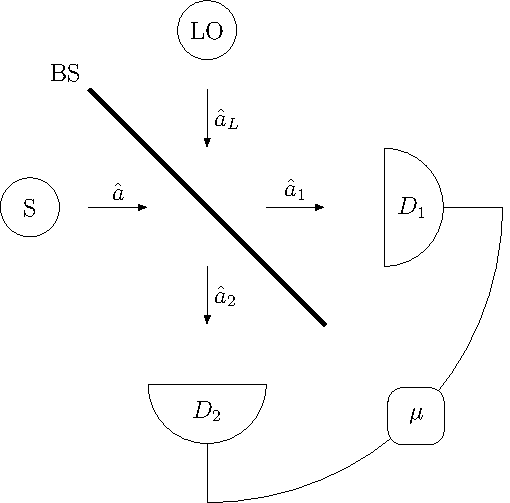
\includegraphics[width=0.75\linewidth]{pics/schemes/homodyne.pdf}
    \caption{Standard scheme of a homodyne receiver. S is the source of the signal mode $\hat{a}$, LO is the source of the reference mode $\hat{a}_{L}$, and BS is the beam splitter with transmission and reflection coefficients {$C=\cos\theta$ and $S=\sin\theta$}, respectively. The photodetectors have quantum efficiencies $\eta_{1}$ and $\eta_{2}$, and $\delta m$ is the photon count difference.}
    \label{fig:homodyne}
\end{figure}

\section{Homodyne detection scheme}\label{sec-homodyne}
{POVM of $m$ photon counts $\hat P_m$ for non-ideal detector of quantum efficiency $\eta$ is given by{~\cite{kelley1964theory}}},
\begin{equation}
    \hat{P}_m=:\frac{(\eta \hat{n})^me^{-\eta \hat{n}}}{m!}:, \label{eq:hpm}
\end{equation}
where $\hat{n}=\hat{a}^\dag\hat{a}$ is the number operator and $:\ :$ designates normal order. {We are ignoring dark counts, because including them is simply a shift of the dependency in the form $\hat{n}+\nu$}.  Since events of registation photon counts $m_1$ and $m_2$ are independent, POVM of the homodyne measurement scheme  (see Fig.~\ref{fig:homodyne}) is a product of POVMs given by Eq.{~\eqref{eq:hpm}} with appropriate indices (See e.g.{~\cite{vogel1993statistics}}),
\begin{equation}
    \hat{P}_{m_1,m_2}=\langle\hat{P}_{m_1,m_2}\rangle =
    :\prod_{l=1}^2\frac{(\eta_l\hat{n}_l)^{m_l}}{m_l!}
    e^{-\eta_l\hat{n}_l}
    :,
\end{equation}
{and the probability of detecting $m_1$ and $m_2$ photon counts is given by averaging this POVM,}
\begin{equation}
    P_{m_1,m_2}=\langle\hat{P}_{m_1,m_2}\rangle =\left\langle
    :\prod_{l=1}^2\frac{(\eta_l\hat{n}_l)^{m_l}}{m_l!}
    e^{-\eta_l\hat{n}_l}
    :
    \right\rangle.\label{eq:h-sred}
\end{equation}
{Hereinafter we will assume both signal and LO to be in coherent states to simplify our analysis, returning to the case of non-coherent signal later in this section.}

{To obtain transformed amplitudes we will use the unitary BS transform} 
\begin{equation}
    \hat{R}_\theta=\begin{pmatrix}
C&S\\-S&C
\end{pmatrix},
\end{equation}
{where we have introduced the following designations:}
\begin{align}
\begin{split}
    \cos\theta&\equiv C,\\
    \sin\theta&\equiv S.
\end{split}
\end{align}
{From the BS transform we may obtain the relations between input and output as follows:}
\begin{equation}
    \begin{pmatrix}
\hat{a}_1\\\hat{a}_2
\end{pmatrix}=
\hat{R}_\theta
\begin{pmatrix}
\hat{a}\\\hat{a}_L
\end{pmatrix}=
\begin{pmatrix}
C\hat{a}+S\hat{a}_L\\
-S\hat{a}+C\hat{a}_L
\end{pmatrix}, \label{eq:h-BS}
\end{equation}
{from which we obtain the transformed amplitutes as}
\begin{align}
\begin{split}
|\alpha_1|&=|C\alpha+S\alpha_L|, \\
|\alpha_2|&=|-S\alpha+C\alpha_L|.
\end{split} \label{eq:amplitudes}
\end{align}
Introducing the photon count difference 
\begin{equation}
    \delta m = m_1-m_2,
\end{equation}
we may express the statistical distribution of the photon count difference in a homodyne scheme, denoted $P$, as a product of two Poisson distributions, in the form
\begin{equation}
    P=\sum_{m_2}
\frac{(\eta_1|\alpha_1|^2)^{\delta m+m_2}}{(\delta m+m_2)!}e^{-\eta_1|\alpha_1|^2}
\frac{(\eta_2|\alpha_2|^2)^{m_2}}{m_2!}e^{-\eta_2|\alpha_2|^2}.
\label{eq:poisson}
\end{equation}
By performing the $m_2$ summation we may express $P$ as ~\cite{skellam1946frequency}
\begin{equation}
  P=e^{-\eta_1|\alpha_1|^2}e^{-\eta_2|\alpha_2|^2}
\left(\frac{\eta_1|\alpha_1|^2}{\eta_2|\alpha_2|^2}\right)^{\frac{\delta m}{2}}
I_{\delta m}\left(2\sqrt{\eta_1\eta_2|\alpha_1|^2|\alpha_2|^2}\right),\label{eq:accurate}
\end{equation}
where $I_k(z)$ is the modified Bessel function of the first kind. %\hl{While we may work with Eq.{~\eqref{eq:accurate}} and use Gaussian approximation of Bessel function (an older approach introduced in{~\cite{freyberger1993photon}}), our results suggest that it is better to use Gaussian approximation of the Poisson distribution, given by Eq.{~\eqref{eq:poisson}} due to POVMs' domain of definition. The first approach ("Bessel approximation") and the problem it causes explained further in Appendix{~\ref{app:bessel}}, and the second approach ("Gaussian approximation") is used in this section.}
\hl{Our findings reveal that the approach of approximating the Skellam distribution using the asymptotic expansion of the modified Bessel function of the first kind is not applicable for POVM construction in the asymmetrical case, which we discuss in Appendix{~\ref{app:bessel}}.}

It is straightforward to show that the Poisson distribution of a discrete variable $x$ with mean $\lambda$ can be approximated by the normal distribution of a continuous variable $x$ with both mean and variance equal to $\lambda$ when $\lambda \gg 1$. Applying this approximation to Eq.{~\eqref{eq:poisson}}, replacing the summation with integration, and using the LO approximation ($|\alpha_L|\gg|\alpha|$) by rewriting the relevant sum and difference as:
\begin{align}
\begin{split}
\eta_1|\alpha_1|^2+\eta_2|\alpha_2|^2&=\left[\eta_1S^2+\eta_2C^2\right]|\alpha_L|^2+\left[\eta_1-\eta_2\right]CS|\alpha_L|\langle\hat{x}_\phi\rangle+{\mathcal{O}}\left(\frac{1}{|\alpha_L|}\right),\\
-\eta_1|\alpha_1|^2+\eta_2|\alpha_2|^2&=\left[-\eta_1S^2+\eta_2C^2\right]|\alpha_L|^2+\left[\eta_1+\eta_2\right]CS|\alpha_L|\langle\hat{x}_\phi\rangle+{\mathcal{O}}\left(\frac{1}{|\alpha_L|}\right),
\end{split}
\label{eq:small-o}
\end{align}
where
\begin{equation}
    \langle\hat{x}_\phi\rangle={2\Re\alpha e^{-i\phi_L}}
\end{equation}
is the average of the phase-rotated quadrature operator of the signal
mode, defined as
\begin{equation}
\hat{x}_\phi=\hat{a}e^{i\phi}+\hat{a}^\dag e^{-i\phi},
    \label{eq:quad-op}
\end{equation}
we obtain the Gaussian approximation for Eq.~\eqref{eq:accurate}, denoted $P_G$,
\begin{multline}
    P_G=\frac{1}{\sqrt{2\pi(\eta_1S^2+\eta_2C^2)|\alpha_L|^2}}
    \exp \biggl[-\frac{1}{2}\frac{
\left[\left(\eta_1+\eta_2\right)CS\right]^2}
{\eta_1S^2+\eta_2C^2}
\times\\\times
{\left(\frac{\delta m}{(\eta_1+\eta_2)CS|\alpha_L|}-\frac{\eta_1S^2-\eta_2C^2}{\left(\eta_1+\eta_2\right)CS}|\alpha_L|-\langle\hat{x}_\phi\rangle\right)^2}\biggr],\label{eq:Pgood}
\end{multline}
which may be rewritten in the form
\begin{equation}
{P}_G(x)=\frac{1}{\sqrt{2\pi(\eta_1S^2+\eta_2C^2)|\alpha_L|^2}}
    \exp \biggl[-\frac{1}{2}D{\left(x-\langle\hat{x}_\phi\rangle\right)^2}\biggr],
    \label{eq:Pgood-w-def}
\end{equation}
where designations
\begin{align}
    \begin{split}
        D&\equiv\frac{
\left[\left(\eta_1+\eta_2\right)CS\right]^2}{\eta_1S^2+\eta_2C^2},\\x&\equiv\frac{\delta m}{(\eta_1+\eta_2)CS|\alpha_L|}-\frac{\eta_1S^2-\eta_2C^2}{\left(\eta_1+\eta_2\right)CS}|\alpha_L|.
    \end{split}
    \label{eq:defs-x-D}
\end{align}
have been used. 

We will now construct the POVM corresponding to the Gaussian approximation $P_G$. To do so, we first note that \eqref{eq:Pgood} is the average of the POVM over coherent states,
\begin{equation}
    P_G=\langle\alpha|\hat{P}_G|\alpha\rangle.
\end{equation}
Moreover, in case of ideal scheme, $P_G$ (denoted $P_0$ for $\eta_1=\eta_2=1$ and $\theta=\frac\pi4$),
\begin{equation}
    \label{eq:p-0}
    P_0\left(x\right)\equiv
    \frac{1}{\sqrt{2\pi|\alpha_L|^2}}
    \exp \left[-\frac{1}{2}{\left(\frac{\delta m}{|\alpha_L|}-\langle\hat{x}_\phi\rangle\right)^2}\right],
\end{equation}
coincides with the $Q$-function for phase-rotated quadrature operator with appropriate variable change and normalization constant $|\alpha_L|^{-1}$,
\begin{equation}
    |\langle \alpha|x , \phi \rangle |^2 = \frac{1}{\sqrt{2\pi}}\exp\left[-\frac{1}{2}\left(x  - \langle \hat{x}_\phi\rangle\right)^2\right], 
\end{equation}
where $|x,\phi\rangle$ is the eigenstate of the phase-rotated quadrature operator~\eqref{eq:quad-op}. This means that in the case of the ideal scheme, the POVM is a projector onto $|x,\phi\rangle$, with appropriate normalization constant:
\begin{equation}
    \hat{P}_G=\frac{1}{|\alpha_L|}|x,\phi\rangle\langle x,\phi|,
\end{equation}
which is known. For the asymmetrical case we may write $P_G$ as a convolution of $P_0$ and a normalized Gaussian function $G(x,\sigma)$
\begin{equation}
    P_G\sim\int\mathop{dx'}G(x-x';\sigma)P_0(x'), \label{eq:theform}
\end{equation}
\begin{equation}
G(x, \sigma_D) = \frac{1}{\sqrt{2\pi\sigma_D}}\exp\left[-\frac{1}{2}\frac{x^2}{\sigma_D}\right],
\end{equation}
with $\sigma_D$ to be determined. The proportionality sign present in Eq.~\eqref{eq:theform} is a consequence of integrating with respect to $x'$ but normalizing integrand with respect to $\delta m$ as per Eq.~\eqref{eq:norm}, meaning that normalization constant is the linear factor relating definition of $x$ through $\delta m$. From Eq.~\eqref{eq:Pgood-w-def} we determine the proportionality constant to be $\left[\left(\eta_1+\eta_2\right)CS|\alpha_L|\right]^{-1}$, ensuring that the set of POVM would sum up to identity. This allows us to write the desired POVM as follows:
\begin{equation}
\hat{P}_G= \frac{1}{\left(\eta_1+\eta_2\right)CS|\alpha_L|}\int\mathop{d^2x'}G(x-x',\sigma_D)|x',\phi\rangle\langle x',\phi|.
\label{eq:method-1}
\end{equation}

Since the convolution of two Gaussian functions results in another Gaussian function with its variance being the sum of the variances of the original functions,
\begin{equation}
    \int\mathop{dx'}e^{-\frac{(x-x')^2}{\sigma_D}}e^{-\frac{x{'}^{2}}{\sigma_0}}=\sqrt{\frac{\pi}{\frac{1}{\sigma_D}+\frac{1}{\sigma_0}}}\exp\left[-\frac{x^2}{\sigma_D+\sigma_0}\right],
    \label{eq:conv}
\end{equation}
if we set $\sigma_0=2$ (variance of Gaussian in Eq.~\eqref{eq:p-0}) and
\begin{equation}
     \sigma_D=\frac{2}{D}-2,\label{eq:h-G}
\end{equation}
and substitute these into Eq.~\eqref{eq:conv}, the resulting variance will be $\frac{2}{D}$, as per Eq.~\eqref{eq:Pgood-w-def}. 
{Definition given by Eq.{~\eqref{eq:h-G}} implies that $D\leq1$, so that $\sigma_D\geq0$. It is not difficult to see that this is always satisfied:}
\begin{equation}
    {\max D=\frac{\left(\eta_1+\eta_2\right)^2}{\left(\sqrt{\eta_1}+\sqrt{\eta_2}\right)^2}\leq1.}
\end{equation}
 Therefore, $D\leq1$ for all $\eta_1$, $\eta_2$, and $\theta$, as opposed to the situation described in Appendix{~\ref{app:bessel}}.

We obtain the desired POVM for the Gaussian approximation as:
\begin{equation}
\hat{{P}}_G=\frac{1}{(\eta_1+\eta_2)CS|\alpha_L|}\int \mathop{dx'} G(x-x'; \sigma_D)|x',\phi\rangle\langle x',\phi|,
\label{eq:homodyne-povm}
\end{equation}
Note that 
\begin{equation}
    \lim_{D\to1}G(x,\sigma_D)=\delta(x),
\end{equation}
where $\delta(x)$ is the Dirac $\delta$-function, which is the expected behavior for Eq.~\eqref{eq:theform} to hold in the limiting case of an ideal scheme. Therefore, the constructed POVM is well-defined for all possible parameters of the homodyne scheme.

The ability of the homodyne scheme to reconstruct the quadrature of the state is well known, which is showcased by Eq.~\eqref{eq:homodyne-povm}.

It is worthwhile to assess how accurate $P_G$ is. To do so, the $L^1$ measure is defined as
\begin{equation}
    \mathtt{D}\left(P,{P}_{G}\right)\equiv
    \frac{1}{2}{\sum_{\delta m}
    \left|P -{P}_G\right|}.
\end{equation}

To illustrate the parameter dependency of the exact and approximate statistical distribution, we numerically calculate them using Eq.~\eqref{eq:accurate} and Eq.~\eqref{eq:Pgood}. The resulting distributions are presented in Fig.~\ref{fig:PLACEHOLDER}. For symmetrical variation of parameters $\eta_1$ and $\eta_2$, distributions and distance between distributions $\mathtt{D}$ changes asymmetrically, which is caused by sign change in Eq.~\eqref{eq:amplitudes}. For $\alpha=0$ symmetrical variation of $\eta_1$ and $\eta_2$ yields statistical distributions, both exact and approximate, as mirror-images of each other, with equal $\mathtt{D}$, as expected. Further calculations reveal that global minima of $\mathtt{D}$ coincide with parameters that shift the global maxima of statistical distributions to be at $0$.

A study of the dependence on amplitude parameters is shown in Fig.~\ref{fig:amplitude}. Both curves behave as expected: monotonic increase for increasing $|\alpha|$ with fixed $|\alpha_L|$ and monotonic decrease for increasing $|\alpha_L|$ with fixed $|\alpha|$. \hl{However, note that for the LO amplitude deviation it becomes significant that the function {\eqref{eq:Pgood}} is normalized in the sense of}
\begin{equation}
    {\sum_{\delta m}
    P_G
    %(x)
    =1,}
    \label{eq:norm}
\end{equation}
\hl{since the normalization constant of the function is dependent on $|\alpha_L|$. Rigorously, re-normalizing the function to $1$ is always needed due to us dealing with finite amplitude of LO, therefore we will always re-normalize the distribution numerically.}
In Fig.~\ref{fig:amplitude}b we may see that approximation is still adequate even when re-normalization of $P_G$ to $1$ is needed. Local maxima and minimas are present as well. \hl{Adequence of Gaussian approximation with numerical re-normalization is an oddity of weak signal amplitude $|\alpha|\ll\left[2(\eta_1S^2+\eta_2C^2)\right]^{-\frac{1}{2}}$.}
%This is caused by significance of discritization  for these parameters,  Degeneration is also causing the presented local minima. This behaviour is presented only for weak signals so that $|\alpha|<\sqrt{(\eta_1S^2+\eta_2C^2)}$, otherwise distance between numerically normalized distribution and exact distribution is greater than for normalized.

We may also plot the distance between distributions as a function of deviation from the ideal scheme, defined by the relation
\begin{equation}
        \delta\theta\equiv\frac{\pi}{4}-\theta,
\end{equation}
or as a function of $\eta_1$ ($\eta_2$) with fixed $\eta_2$ ($\eta_1$). The results are presented in Fig.~\ref{fig:delta-theta} and Fig.~\ref{fig:delta-eta}. We can see that the global minima of these functions depend on $\delta\theta$ as well as $\eta_1$ and $\eta_2$, shifting from zero for asymmetrical parameters. We may once again see that minimal distance between statistical distributions for non-ideal parameters corresponds to shifting global maxima of statistical distributions to be at $0$ -- this is seen by curves having global minima not at $\delta\theta=0$ and $\eta_{1}=1$ or $\eta_{2}=1$ respectively. 
We may also see the agreement at critical points $\pm\frac{\pi}{4}$ seen at Fig.~\ref{fig:delta-theta}. \hl{This is expected behaviour. While rigorously we cannot apply strong LO approximation for these critical points, since the condition $\eta_1|\alpha_1|^2\gg1$  (or $\eta_2|\alpha_2|^2\gg1$ ) does not hold in these cases, at these points one of the transformed amplitudes detected is proportional to only $|\alpha_L|$ and the other only to $|\alpha|$ (See Eq.{~\eqref{eq:amplitudes})}. Since $|\alpha_L|\gg|\alpha|$, if efficiencies of the detector arms detecting $\sim|\alpha_L|$ amplitude are equal, both exact and approximate distributions are rendered essentially the same, resulting in the same distance between them. Which is why, for example, the blue curve in Fig.{~\ref{fig:delta-theta}}, plotted for  $\eta_1=1, \eta_2=0.5$ agrees with the black curve, plotted for the relevant parameter $\eta_1=1$, at point $\delta\theta=-\frac{\pi}{4}$ -- transformed amplitudes are given by $\eta_1|\alpha_L|$ and $\eta_2|\alpha|$, and $\eta_1$ are equal for them. Likewise, the blue curve agrees with the green curve, plotted for the relevant parameter $\eta_2-0.5$, at point $\delta\theta=\frac{\pi}{4}$, correspoinding to the detector with efficiency $\eta_2$. The same logic applies to the orange curve.}
Monotonically increasing curves seen in Fig.~\ref{fig:delta-eta} correspond to the shifting of global maxima of statistical distributions to be further from $0$. Asymmetry between curves for symmetrical parameter change is again explained by sign change in Eq.~\eqref{eq:amplitudes}. 

\begin{figure}
    \centering
     \begin{minipage}[c]{.45\linewidth}
 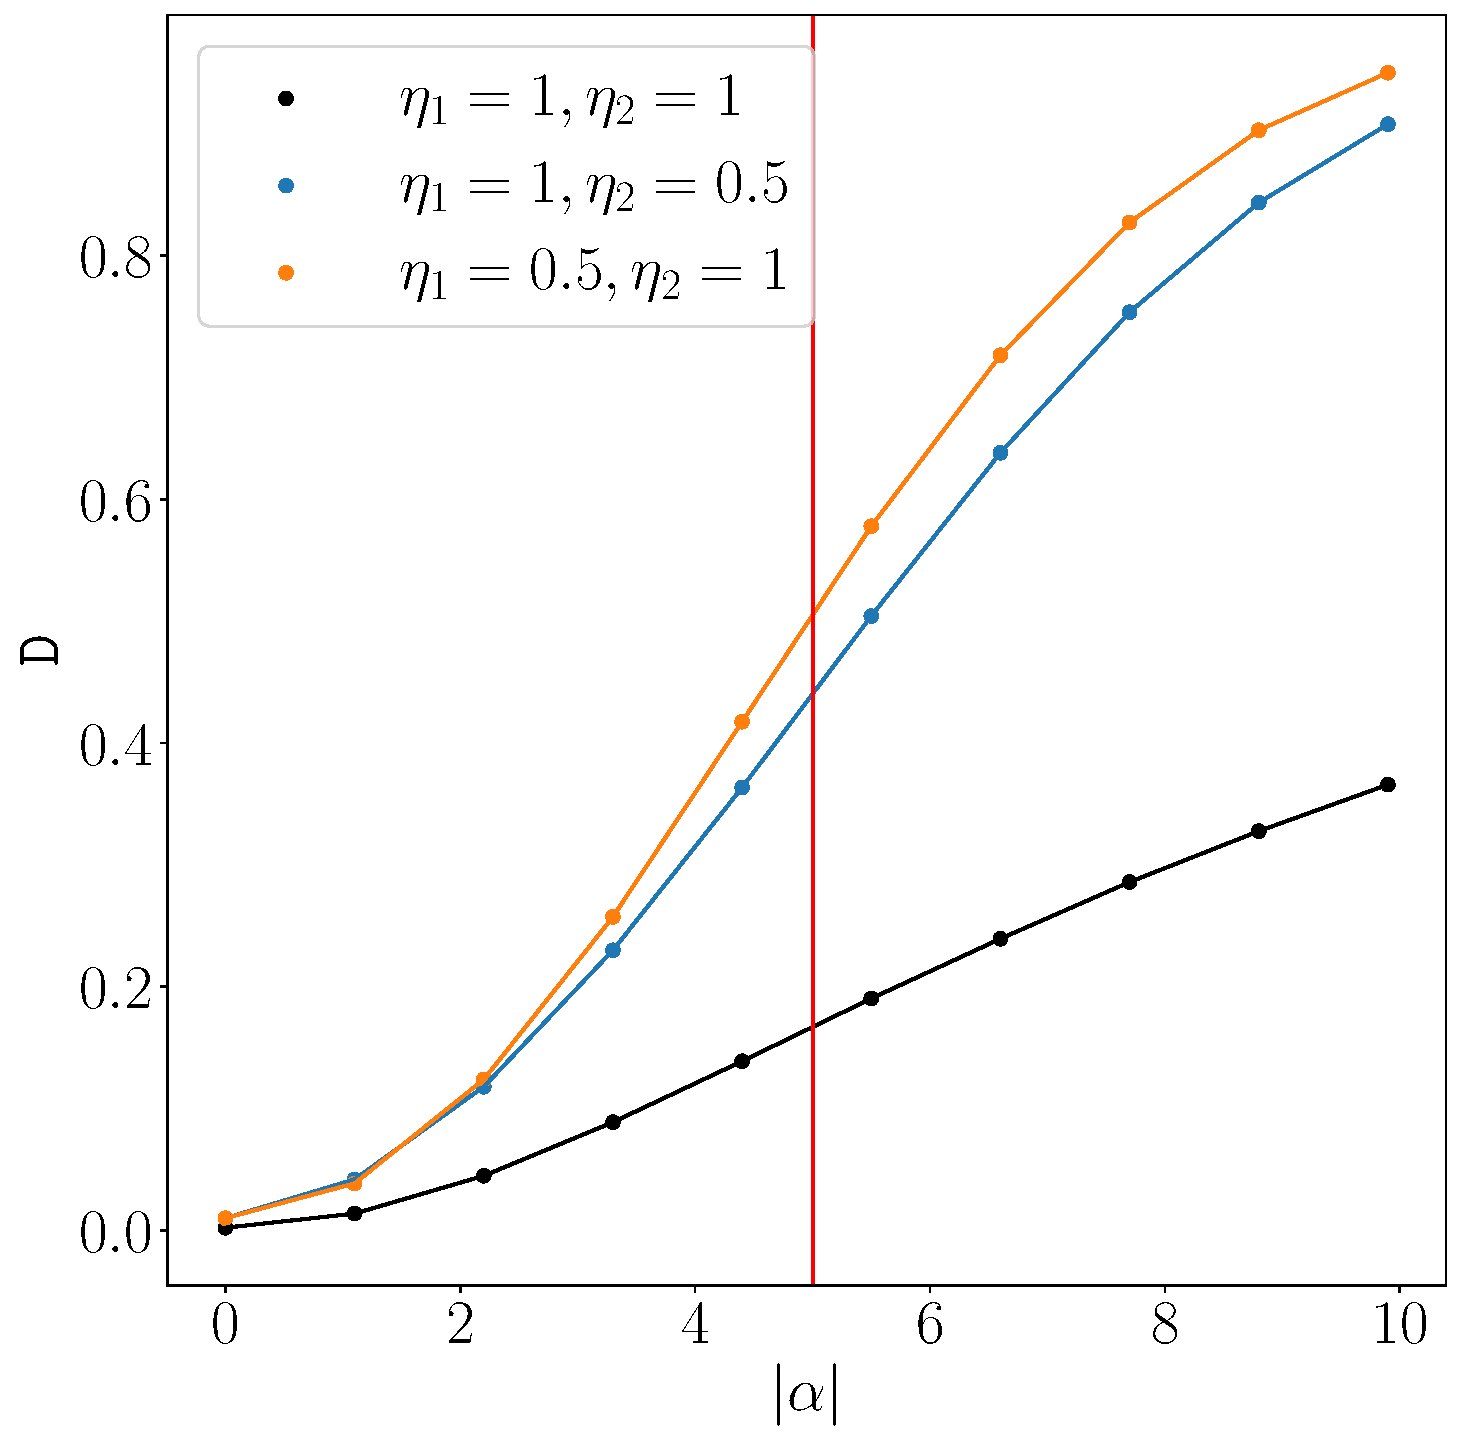
\includegraphics[width=\linewidth]{pics/homodyne/ED = ED(a)_5eta.pdf}
\subcaption[]{$|\alpha_L|=5$}
\end{minipage}
\hfill
\begin{minipage}[c]{.45\linewidth}
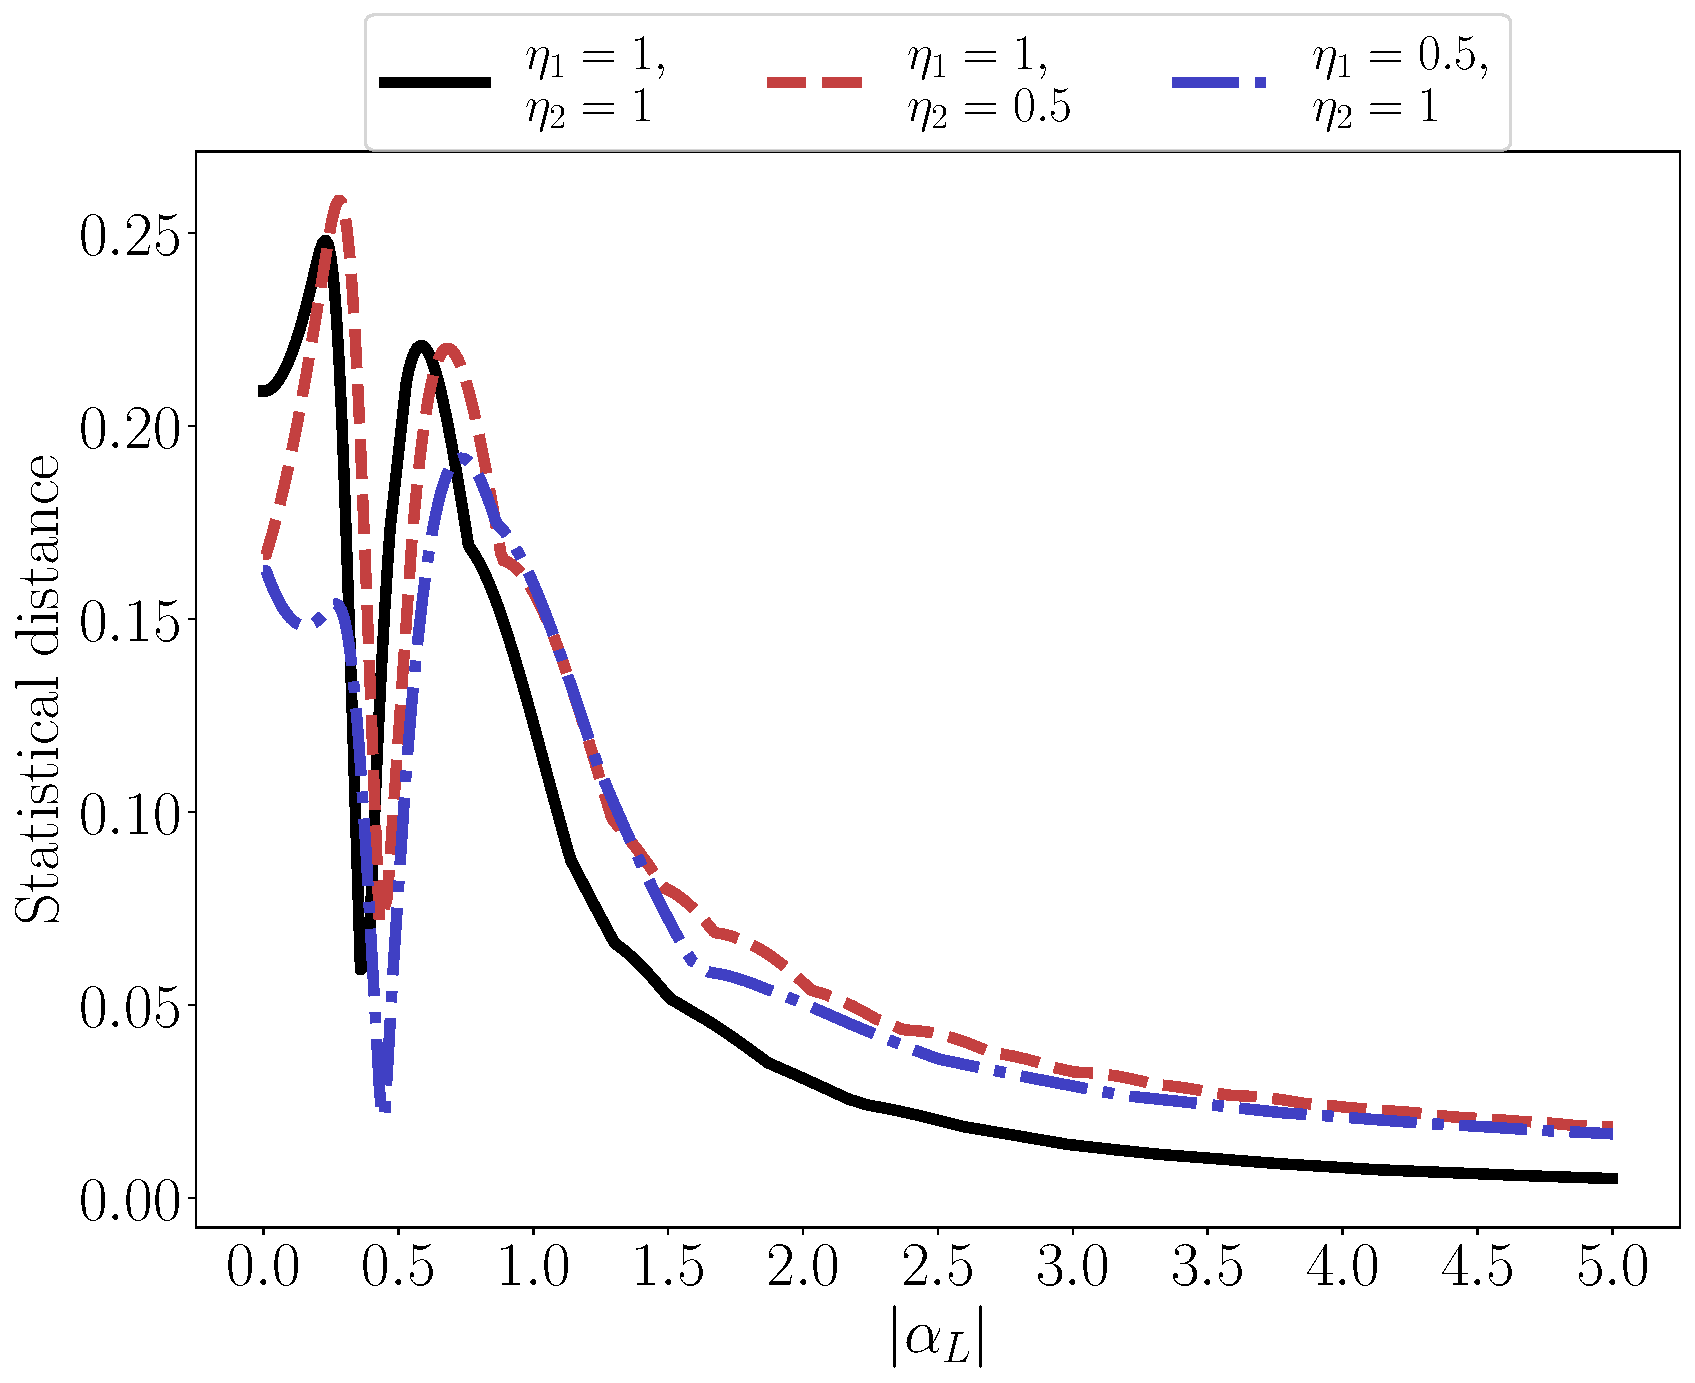
\includegraphics[width=\linewidth]{pics/homodyne/ED = ED(al).pdf}
\subcaption[]{$|\alpha|=0.1$}
        \end{minipage}
    \caption{
    Numerically calculated distance between the exact distribution and the Gaussian approximation as a function of (a) signal amplitude and (b) LO amplitude for different parameters of the beam splitter and detector efficiencies in the asymmetrical homodyne scheme. Red vertical line signifies $|\alpha|=|\alpha_L|$. \hl{More points are added when we expect anomalous behaviour.}
    }\label{fig:amplitude}
\end{figure}

\begin{figure}
    \centering
    \begin{minipage}[c]{.45\linewidth}
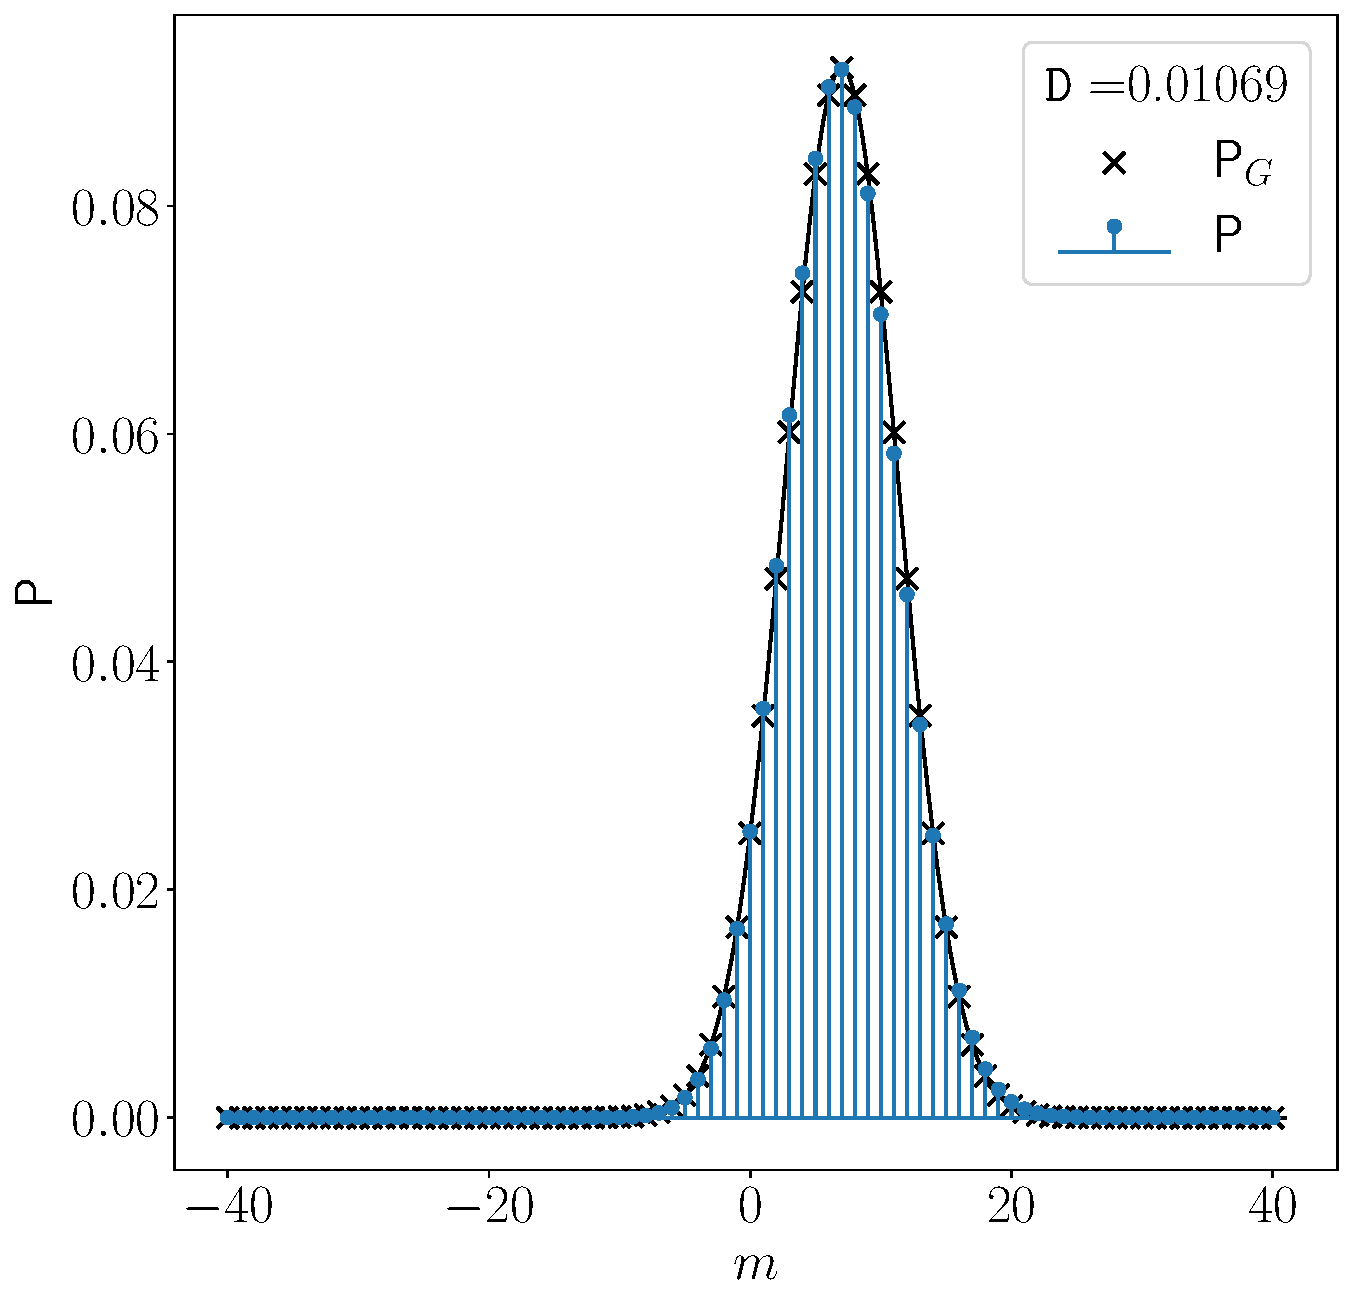
\includegraphics[width=\linewidth]{pics/homodyne/eta1=1, eta2=0.5, theta=1.0.pdf}
\subcaption[]{$\eta_1=1,\eta_2=0.5$}
        \end{minipage}
\hfill
        \begin{minipage}[c]{.45\linewidth}
 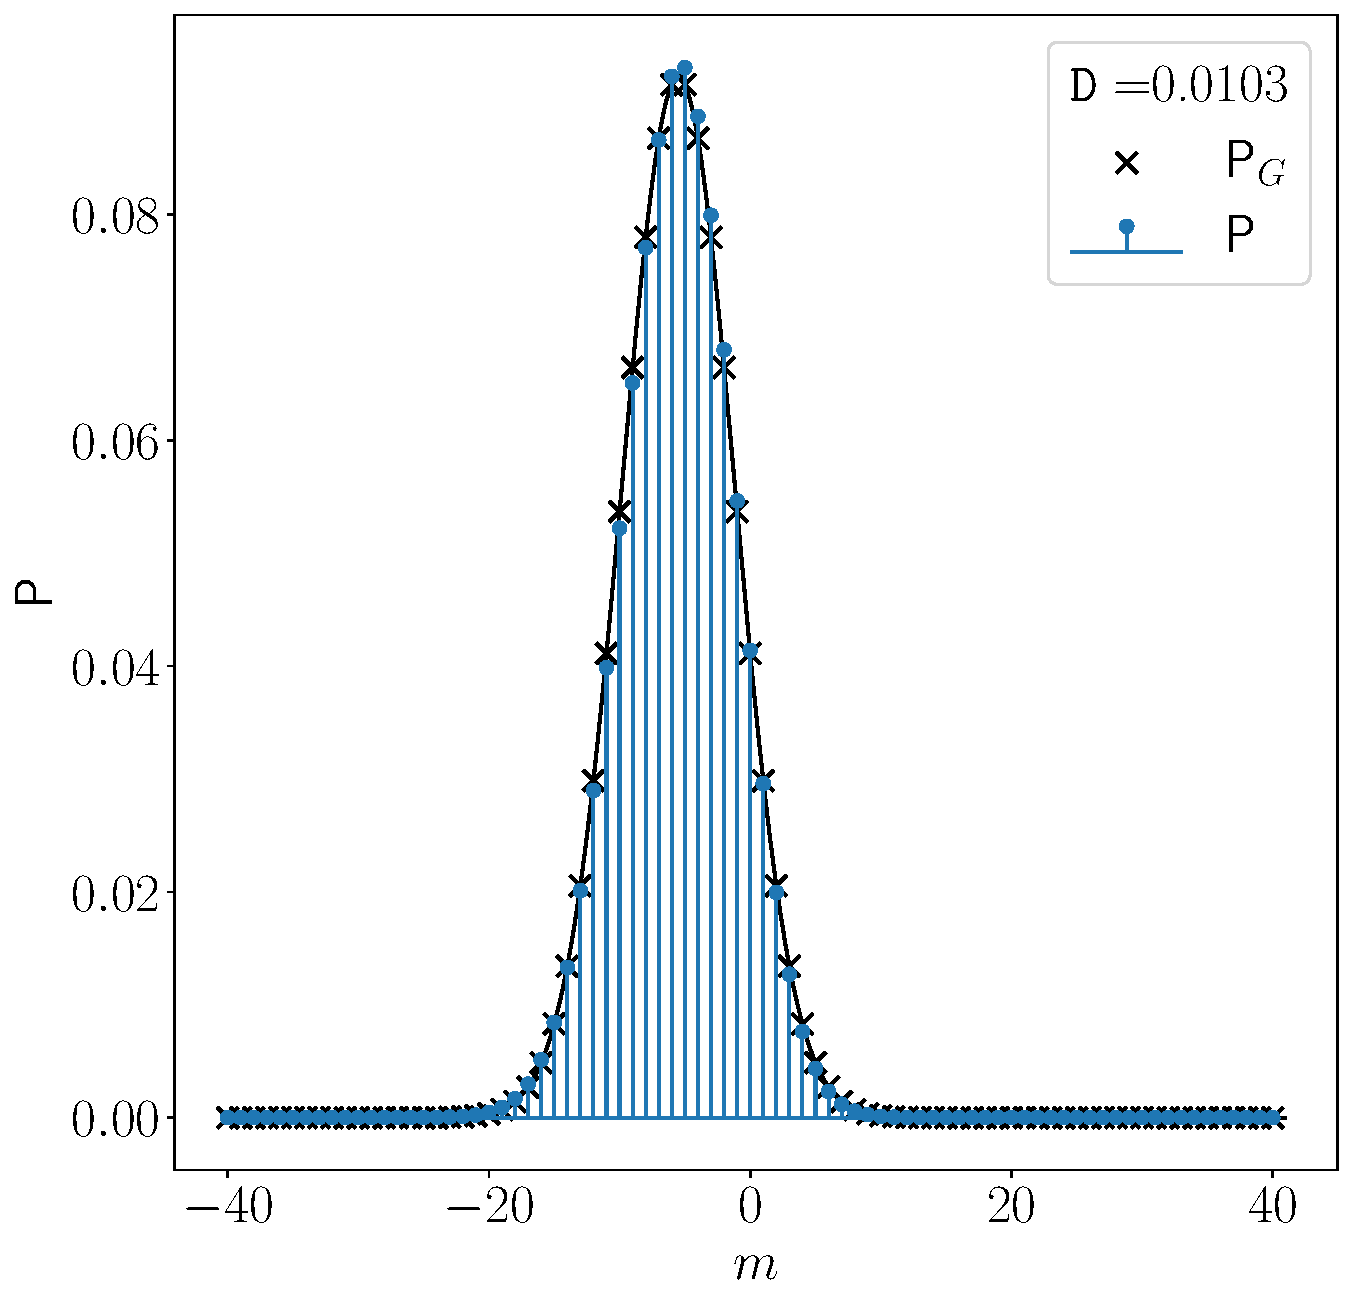
\includegraphics[width=\linewidth]{pics/homodyne/eta1=0.5, eta2=1, theta=1.0.pdf}
\subcaption[]{$\eta_1=0.5,\eta_2=1$}
\end{minipage}
    \caption{
    Numerically calculated statistical distributions of photon count difference in the asymmetrical homodyne scheme, given by  Eq.~\eqref{eq:accurate} (blue) and Eq.~\eqref{eq:Pgood} (black) for different parameters of quantum efficiencies, with $|\alpha|=0.1$ and $|\alpha_L|=5$. Shifting of global maxima for approximation is explained by the term proportional to $|\alpha_L|$ in Eq.~\eqref{eq:Pgood}, and for exact formulae by the terms proportional to $|\alpha_L|$ in Eq.~\eqref{eq:accurate}, which is better seen as the argument of the modified Bessel function in Eq.~\eqref{eq:Skellam}. Asymmetry in distributions with symmetrical parameter variation is explained by dependence on $|\alpha|$. Note the significant difference in $\mathtt{D}$.
    }\label{fig:PLACEHOLDER}
\end{figure}

\begin{figure}
    \centering
    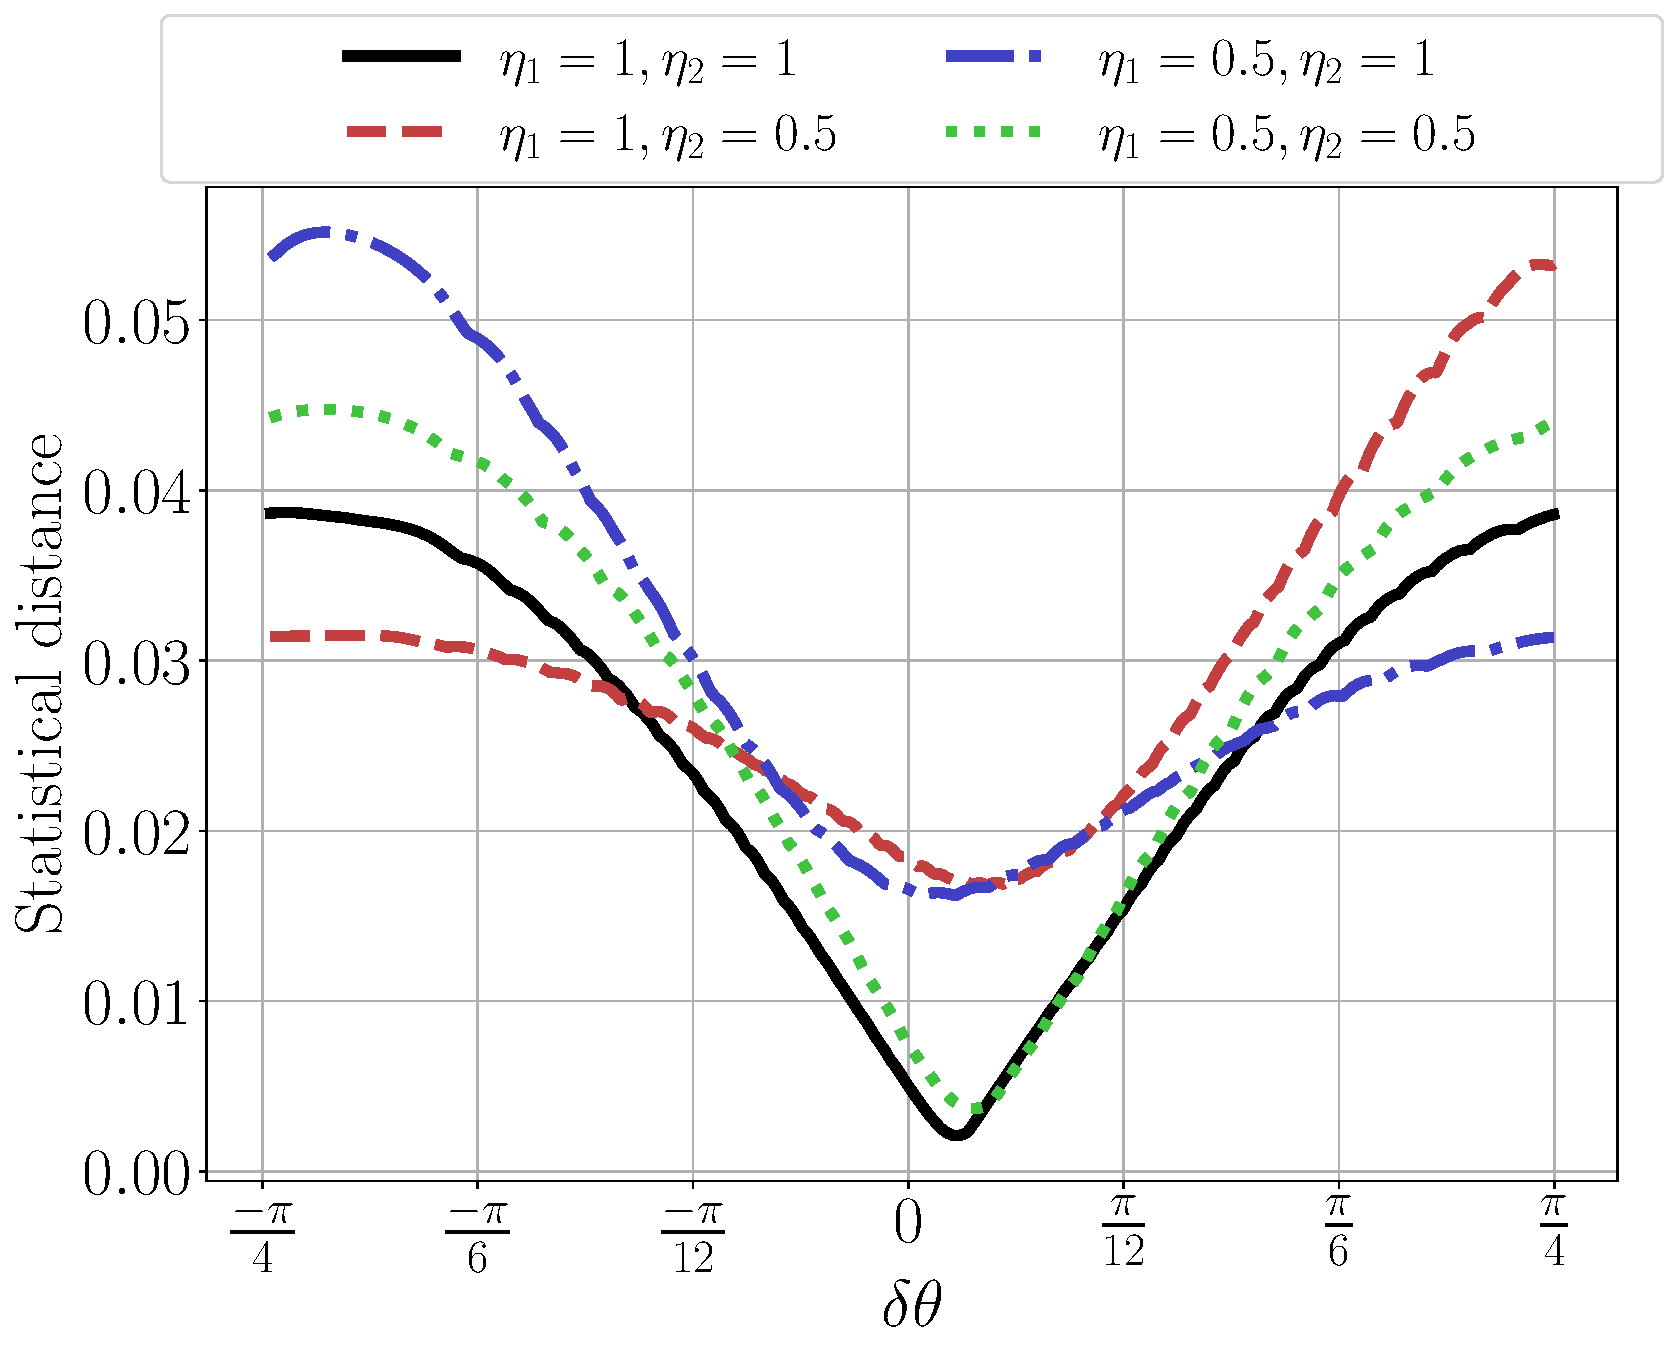
\includegraphics[width=0.75\linewidth]{pics/homodyne/full.pdf}
    \caption{Numerically calculated distance between the exact distribution of photon count difference in the asymmetrical homodyne scheme and its Gaussian approximation as a function of deviation from a balanced beam splitter for different detector efficiencies, with $|\alpha|=0.1$ and $|\alpha_L|=5$. Shifting of global minima $\mathtt{D}$ coincides with parameters that shift the global maxima of statistical distributions to be at $0$.}% Note the agreement at critical points $\pm\frac{\pi}{4}$ \hl{between some of the curves} -- \hl{this is caused by full reflection (transmission) into one output port of the scheme, which makes statistical distributions at these points essentially the same for equal relevant efficiency parameters}.}
    \label{fig:delta-theta}
\end{figure}

\begin{figure}
    \centering
    \begin{minipage}[c]{.45\linewidth}
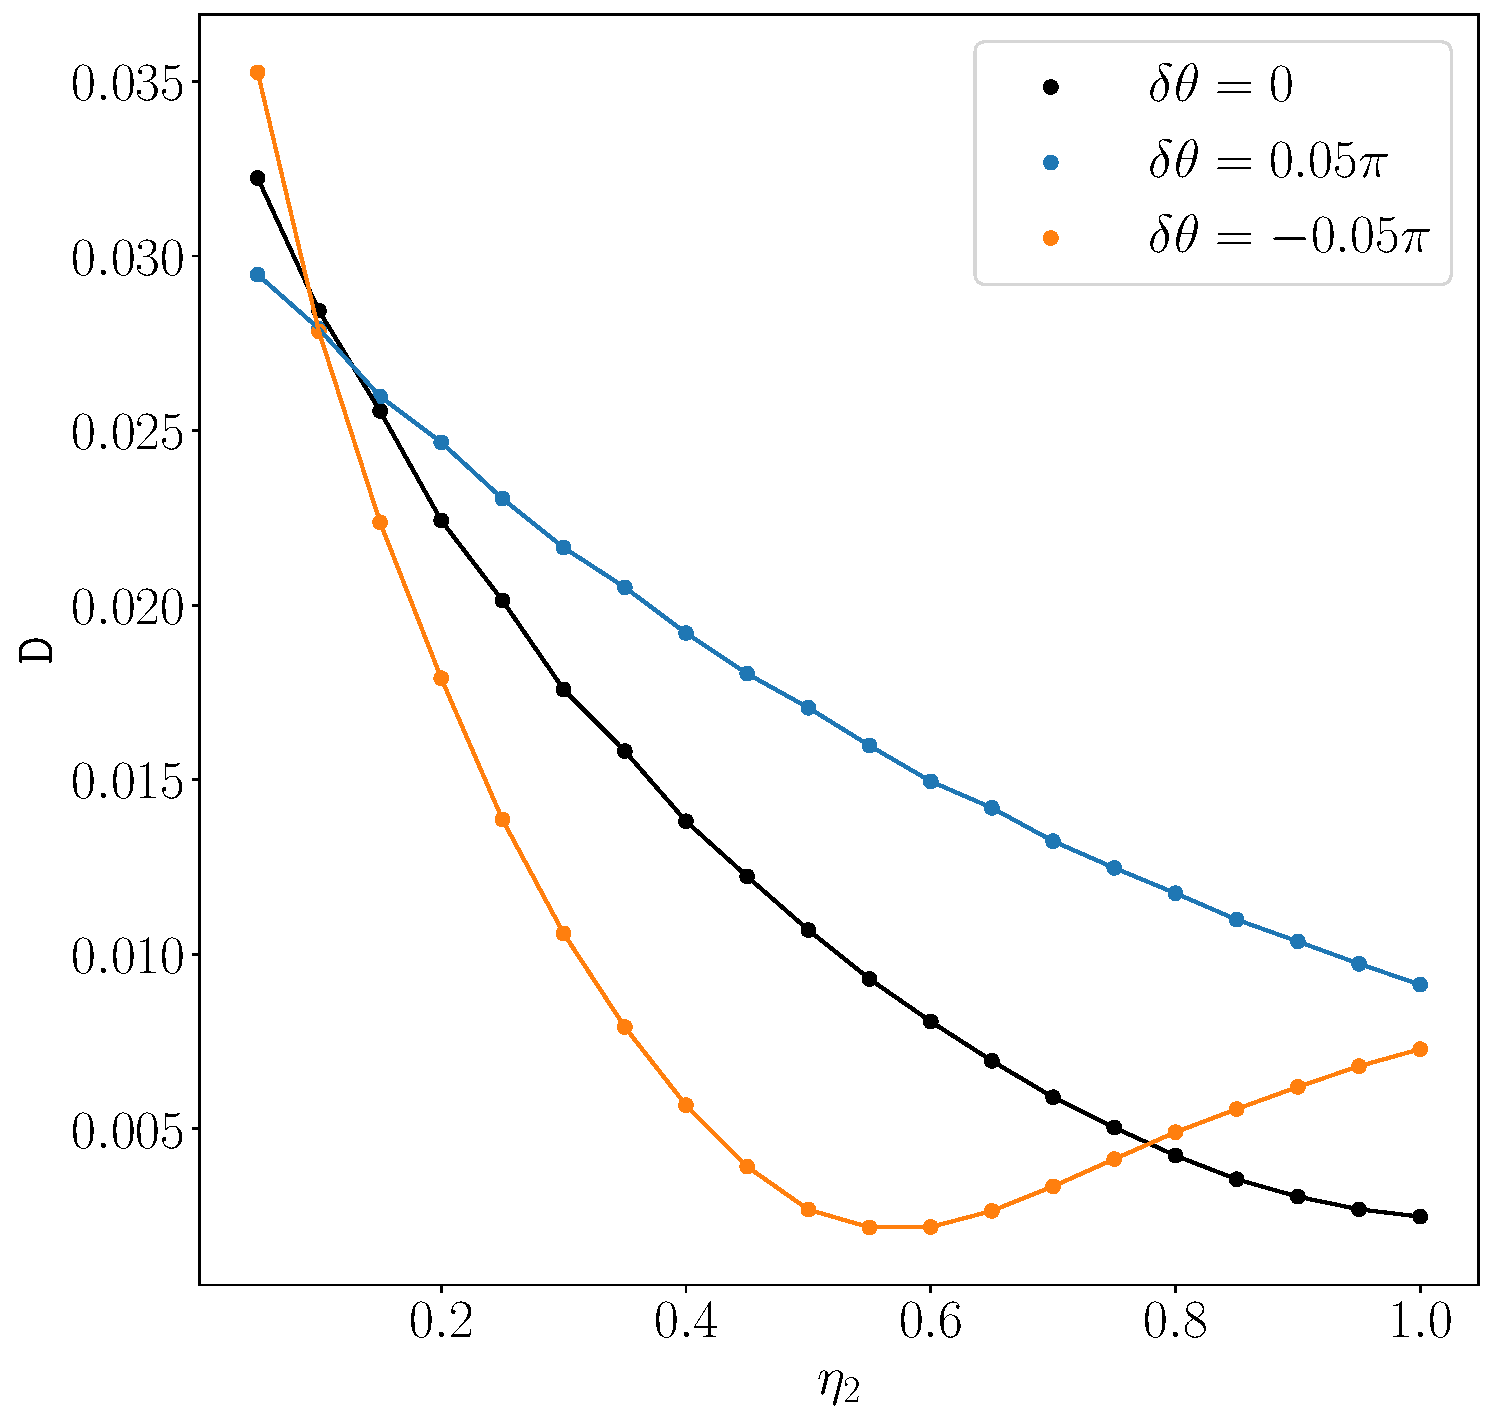
\includegraphics[width=\linewidth]{pics/homodyne/full1.pdf}
\subcaption[]{$\eta_1=1$}
        \end{minipage}
\hfill
        \begin{minipage}[c]{.45\linewidth}
 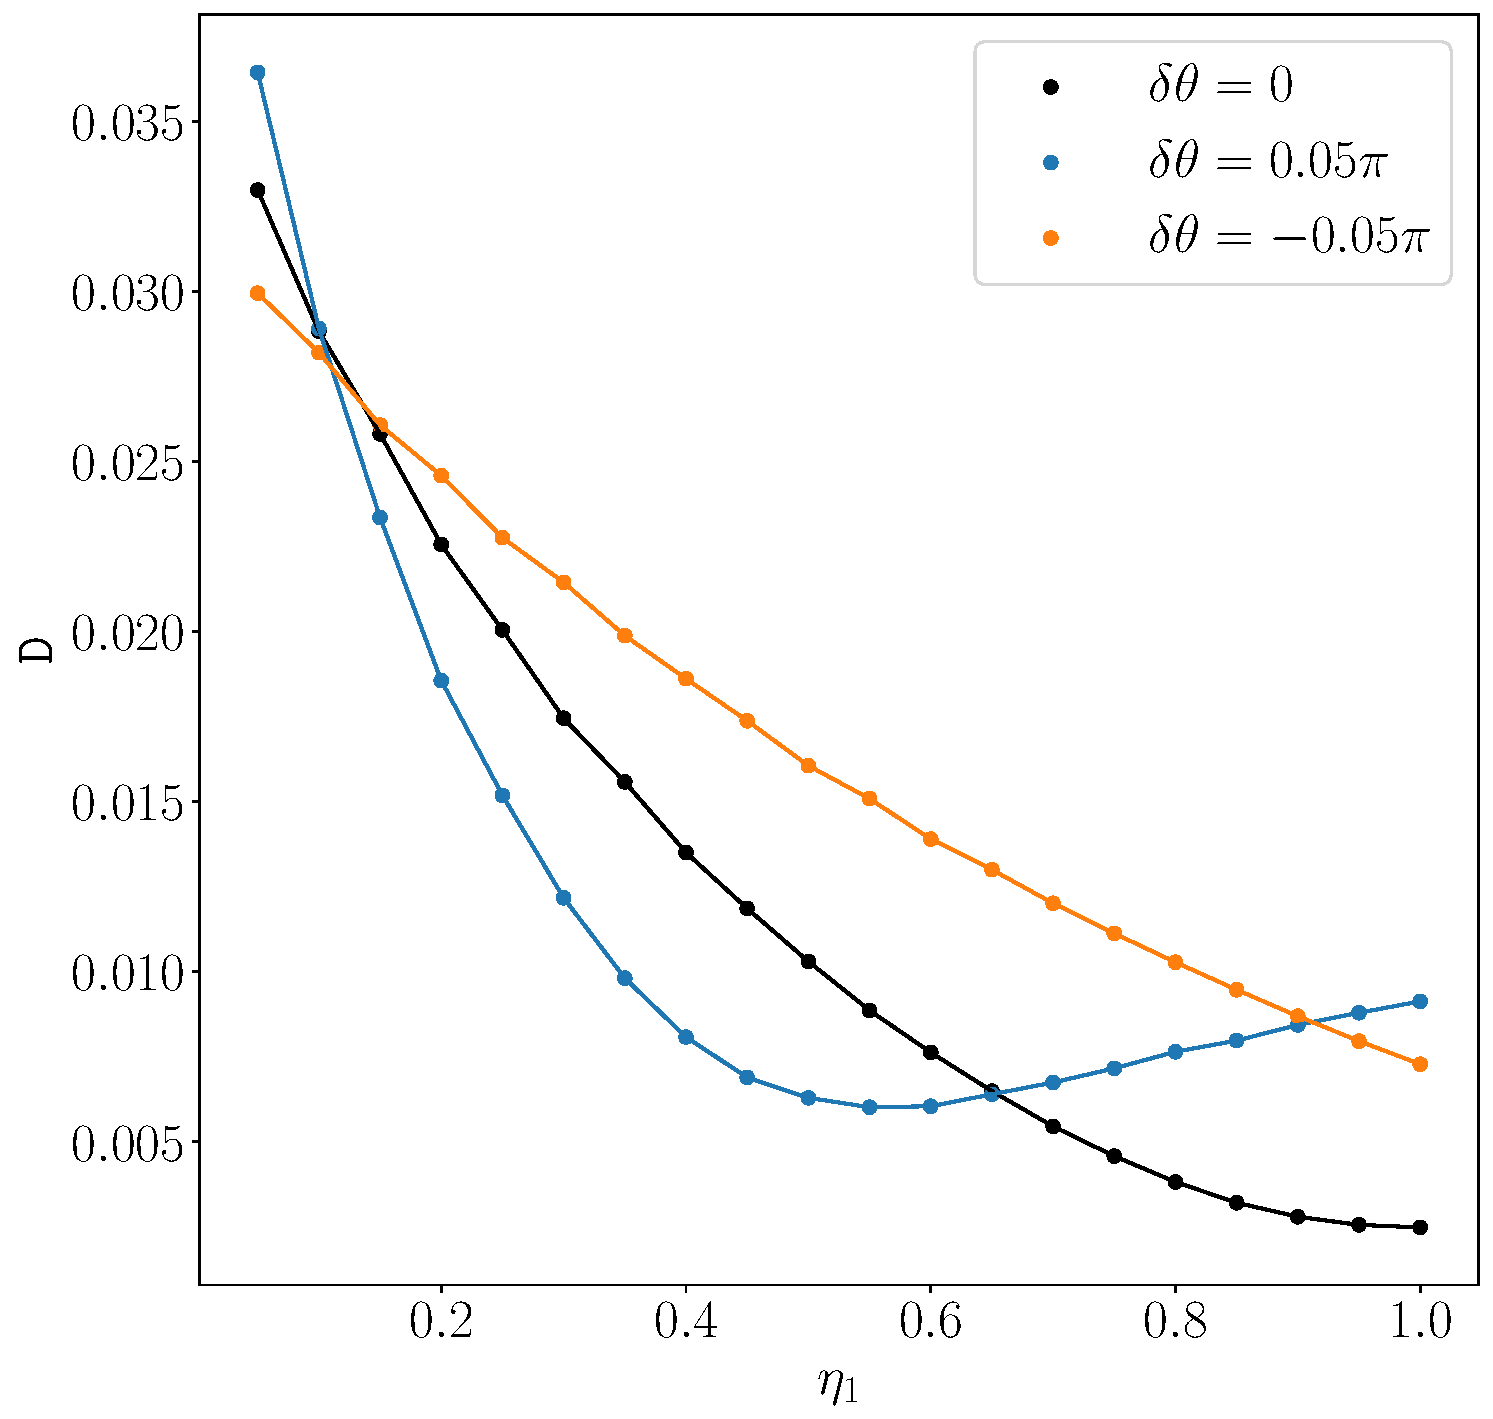
\includegraphics[width=\linewidth]{pics/homodyne/full2.pdf}
\subcaption[]{$\eta_2=1$}
\end{minipage}
    \caption{
    The numerically calculated distance between the exact distribution of photon count difference in the asymmetrical homodyne scheme and its Gaussian approximation as a function of deviation from equal detector efficiencies for different beam splitter parameters, with $|\alpha|=0.1$ and $|\alpha_L|=5$. For curves with global minima not at $\eta_1=1$ or $\eta_2=1$, parameters of both $\eta_1$ and $\eta_2$ coincide with parameters which shift the global maxima of statistical distributions to be at zero.
    }\label{fig:delta-eta}
\end{figure}

A similar methodology may be performed for a non-coherent signal state. To do so, both $P$ and $P_G$ need to be averaged with relevant $P$-function $P_\psi$, yielding relevant distributions $P^\psi$ and $P_G^\psi$,
\begin{equation}
P^\psi=\int \mathop{d^2\alpha} P_{\psi}(\alpha)P(\alpha).
\end{equation}

Here we present the results for the Fock state with $n=1$. Its $P$-function has the form \cite{vogel2006quantum}
\begin{equation}
    P_{(n)}(\alpha)=
    \sum_{k=0}^n \binom{n}{k}\frac{1}{k!} \partial_{\alpha}^k\partial^k_{\alpha^*}\delta(\alpha).
\end{equation}
The dependency of the distance between exact and approximate distributions on the efficiency of the detectors is very much like one for the coherent state and is therefore not presented. Results for dependency on $\delta\theta$ are presented in Fig.~\ref{fig:fock}. We may observe the global minima as always at $0$, and local minima at critical points. 
Global maxima are dependent on parameters of efficiency, and symmetrical parameter variation results in symmetrical distributions. \hl{Moreover, the same agreement at critical points between some of the curves as presented at Fig.{~\ref{fig:delta-theta}} can be seen -- this effect has the same explanation.} 
\begin{figure}
    \centering
    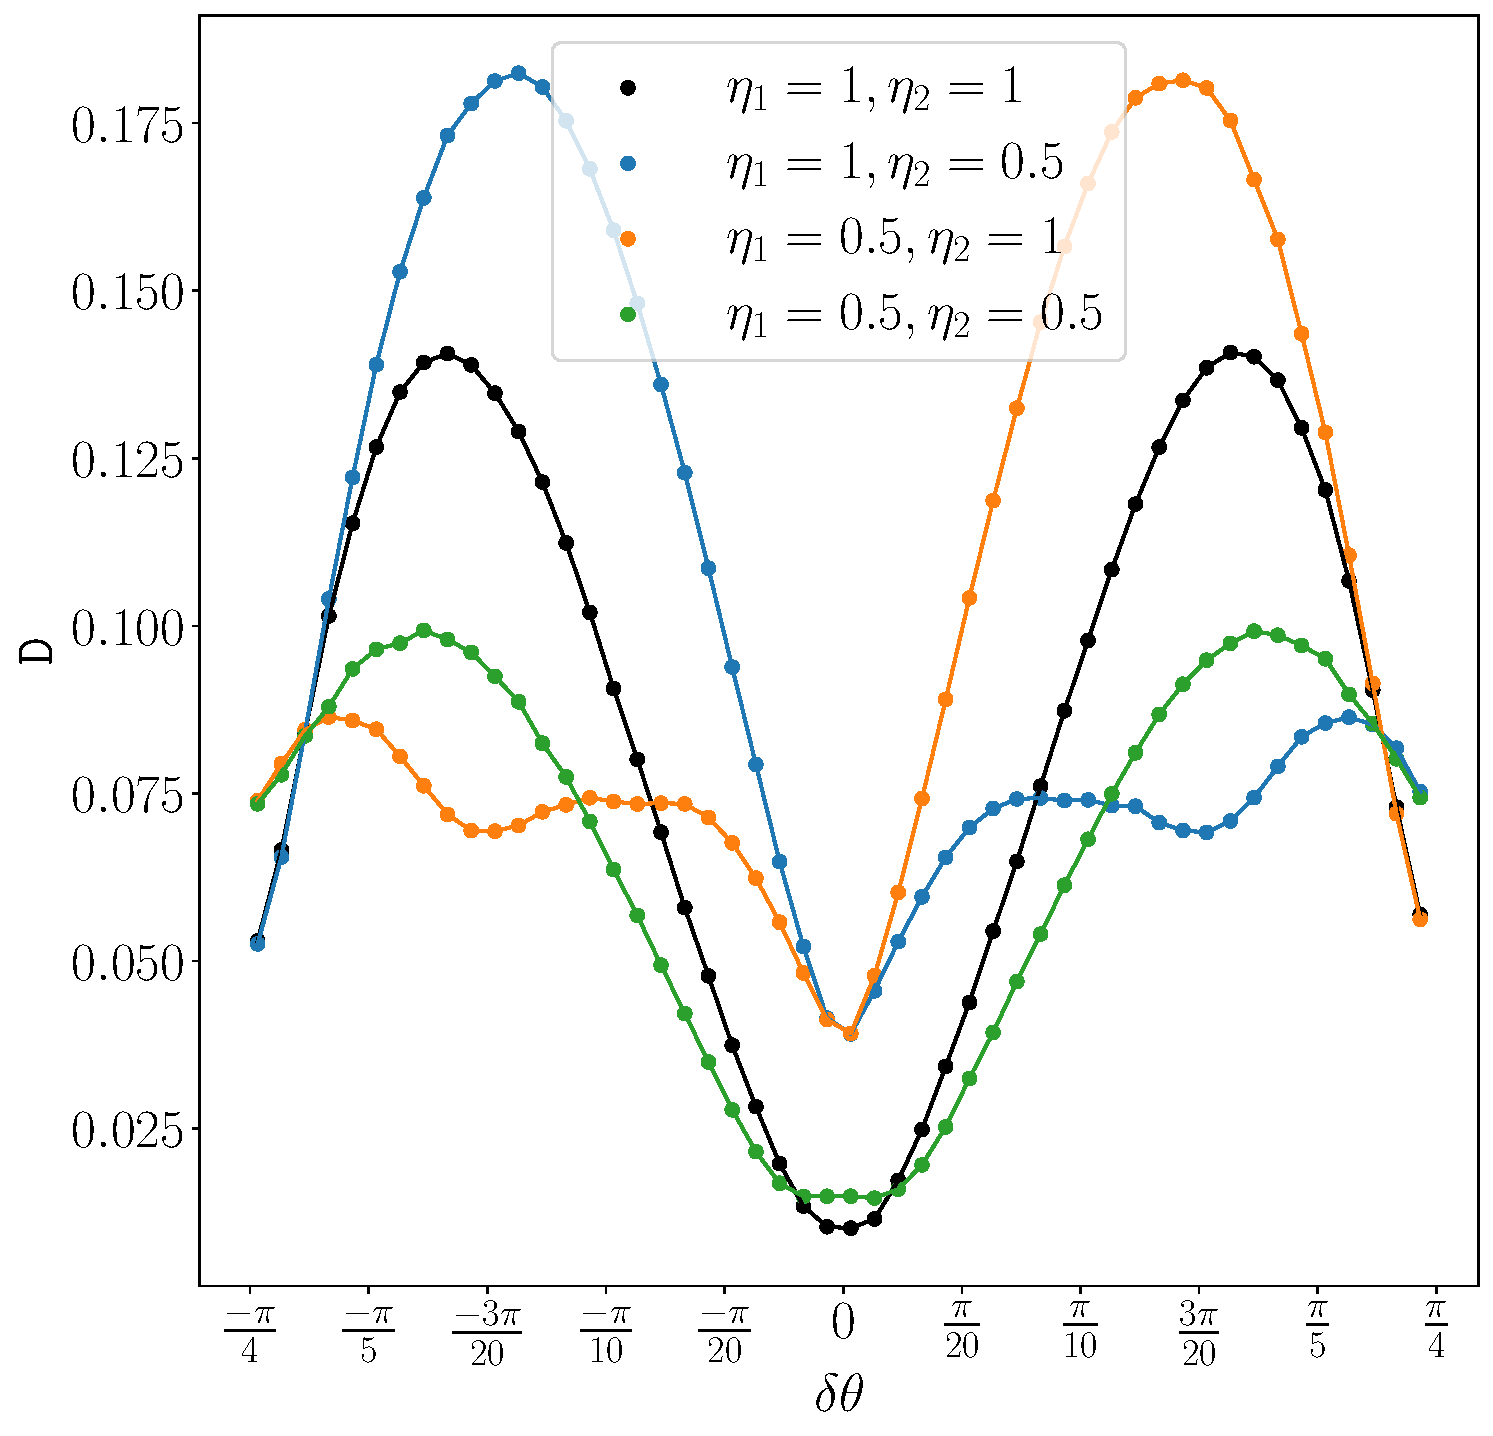
\includegraphics[width=0.75\linewidth]{pics/homodyne/fock.pdf}
    \caption{Numerically calculated distance between the exact distribution of photon count difference in the asymmetrical homodyne scheme and its Gaussian approximation for the single photon signal state as a function of deviation from a balanced beam splitter for different detector efficiencies, with $|\alpha_L|=5$. }%\hl{Note the presence of the same agreement at critical points $\pm\frac{\pi}{4}$ much like the same effect seen at Fig.{~\ref{fig:delta-theta}} -- the same explanation applies here.}}
    \label{fig:fock}
\end{figure}

\begin{figure}
    \centering
    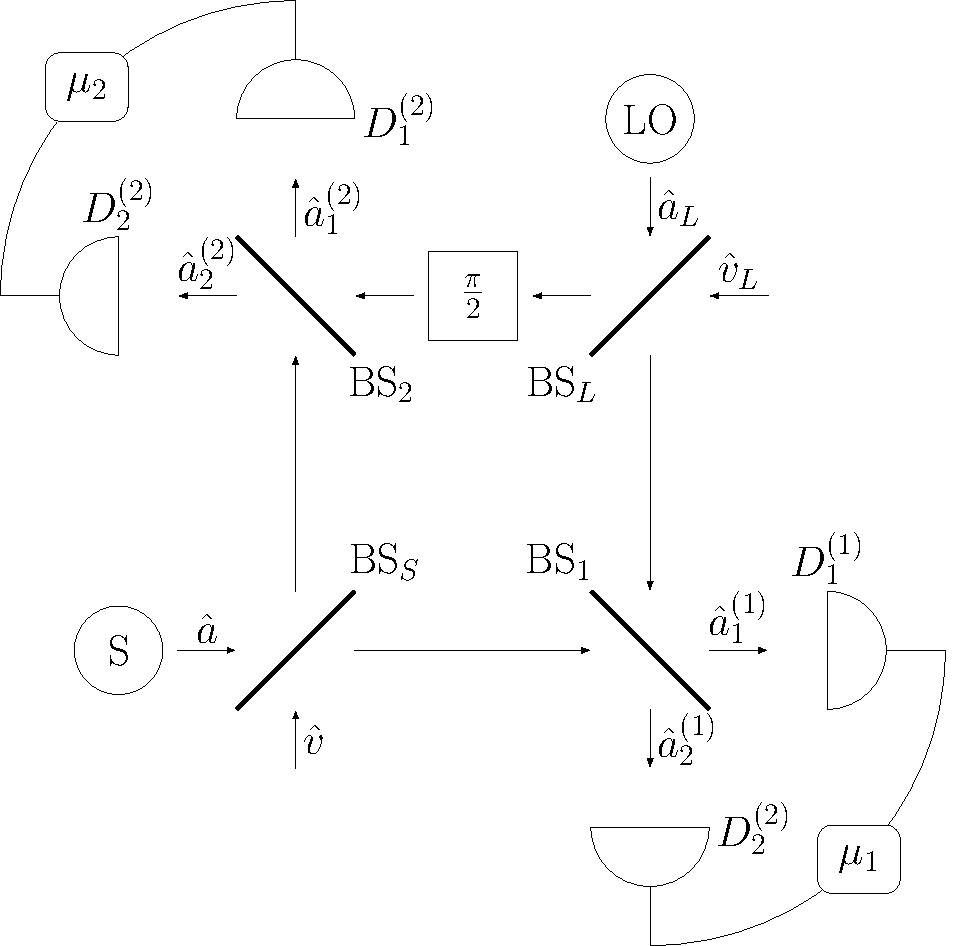
\includegraphics[width=0.75\linewidth]{pics/schemes/double_homodyne.pdf}
    \caption{Scheme of 8-port double homodyne receiver. S is the source of the signal mode $\hat{a}$, LO is the source of the reference mode $\hat{a}_{L}$, and BS$_l$ is the beam splitter with transmission and reflection coefficients $t_l$ and $r_l$, respectively, where $l=1,\ldots,4$. $\frac{\lambda}{4}$ is a half-wave plate. The photodetectors have quantum efficiencies $\eta_{l}$, and $\delta m_l$ is the photon count difference.}
    \label{fig:double-homodyne}
\end{figure}

\section{Double homodyne detection scheme}\label{sec-double-homodyne}

Consider the 8-port double homodyne scheme (Fig.~\ref{fig:double-homodyne}) \cite{lahti2010realistic}. It is known that this measurement scheme allows to reconstruct the $Q$-function of the signal state \cite{Richter:98}, yielding full information about the signal state, which may be used in CV-QKD protocols. It should be noted that the restoration of the state complex amplitude entirely serves as the basis for composable security proofs~\cite{PhysRevLett.93.170504,PhysRevLett.118.200501,pirandola2024improvedcomposablekeyrates,pascualgarcía2024improvedfinitesizekeyrates}. Analogous to Eq.~\eqref{eq:accurate}, the statistical distribution of photon count difference is written as:
\begin{multline}
P= \left(\frac{\eta_1|\alpha_1|^2}{\eta_4|\alpha_4|^2}\right)^{\frac{\delta m_1}{2}}
I_{\delta m_1}\left(2\sqrt{\eta_1\eta_4|\alpha_ 1|^2|\alpha_4|^2}\right)
e^{-\eta_1|\alpha_1|^2}
e^{-\eta_4|\alpha_4|^2}\times\\\times
\left(\frac{\eta_3|\alpha_3|^2}{\eta_2|\alpha_2|^2}\right)^{\frac{\delta m_2}{2}}
I_{\delta m_2}\left(2\sqrt{\eta_2\eta_3|\alpha_ 2|^2|\alpha_3|^2}\right)
e^{-\eta_2|\alpha_2|^2}
e^{-\eta_3|\alpha_3|^2}\label{eq:accurate-dh},
\end{multline}
where
\begin{align}
\begin{split}
    |\alpha_1|&=|
    C_1C_2\alpha
    -S_3S_2\alpha_L|,\\
    |\alpha_2|&=
    |S_1C_4\alpha
    -iC_3S_4\alpha_L|,\\
    |\alpha_3|&=|
     S_1S_4\alpha
    +iC_3C_4\alpha_L|,\\
    |\alpha_4|&=|
    C_1S_2\alpha+
    S_3C_2\alpha_L|.
\end{split}
\end{align}

The approximation method used in the previous section yields the Gaussian approximation
\begin{multline}
P_G=\frac{\biggl[(\eta_1S_2^2+\eta_4C_2^2)(\eta_3C_4^2+\eta_2S_4^2)\biggr]^{-\frac{1}{2}}}{2\pi C_3S_3|\alpha_L|^2}\times\\\times \exp \biggl[-D_1\left(x_1+\frac{\Re\alpha\alpha_L^*}{|\alpha_L|}\right)^2\biggr]\exp \biggl[-D_2\biggl(x_2-\frac{\Im\alpha\alpha_L^*}{|\alpha_L|}\biggr)^2\biggr], \label{eq:Pgood-dh}
\end{multline}
where designations
\begin{align}
    \begin{split}
D_1&=\frac{2(C_1C_2S_2[\eta_1+\eta_4])^{2}}{\eta_1S_2^2+\eta_4C_2^2},\\
    D_2&=\frac{2(S_3S_4C_4[\eta_3+\eta_2])^2}{\eta_3C_4^2+\eta_2S_4^2},
    \end{split}\label{eq:dh-D}
\end{align}
\begin{align}
    \begin{split}
x_1&=\frac{\delta m_1}{2|\alpha_L|C_1C_2S_2S_3[\eta_1+\eta_4]}+\frac{-\eta_1S_2^2S_3^2+\eta_4S_3^2C_2^2}{2C_1C_2S_2S_3[\eta_1+\eta_4]}|\alpha_L|, \\
    x_2&=\frac{\delta m_2}{2|\alpha_L|S_1S_4C_3C_4[\eta_3+\eta_2]}+\frac{-\eta_3C_3^2C_4^2+\eta_2C_3^2S_4^2}{2S_1S_4C_3C_4[\eta_3+\eta_2]}|\alpha_L|
    .
    \end{split}\label{eq:dh-x}
\end{align}
have been introduced. Note that Eq.~\eqref{eq:Pgood-dh} is a product of two functions in the form of Eq.~\eqref{eq:Pgood} (much like Eq.~\eqref{eq:accurate-dh} is a product of two function in the form of Eq.~\eqref{eq:accurate}), meaning approximation quality study in previous section fully applies for this case. Indeed, the difference statistics of the double homodyne scheme is difference statistics of two separate homodyne schemes with quadrature displaced by $\frac{\pi}{2}$, normalized to unity (See Fig.~\ref{fig:dh-statistics}). 

Using the method introduced in the previous section, by comparing Eq.\eqref{eq:Pgood-dh} of the ideal scheme and the $Q$-function of coherent state,
\begin{equation}
    |\langle\beta|\alpha\rangle|^2=\exp\left[-
    (\beta_1-\alpha_1)^2-(\beta_2-\alpha_2)^2
    \right], %ez 2 show
\end{equation}
where for complex numbers we introduced the notation $\alpha=\alpha_1+i\alpha_2$, and introducing 
\begin{align}
\begin{split}
    \sigma_{D_1}\equiv\frac{1}{D_1}-1,\\
    \sigma_{D_2}\equiv\frac{1}{D_2}-1,
\end{split}
\label{eq:dh-G}
\end{align}
we may write $P_G$ in the form
\begin{multline}
    {{P}}_G=\frac{1}{4{\pi}C_3S_3[\eta_1+\eta_4][\eta_3+\eta_2]S_2^2\sqrt{ C_1C_2S_4C_4}|\alpha_L|^2} \int \mathop{dx'_1dx'_2}\times\\\times G(x_1-x_1', \sigma_{D_1})G(x_2-x_2', \sigma_{D_2})|\langle\alpha|e^{-i\phi_L}\left(-x_1'+ix_2'\right)\rangle|^2,%\label{eq:dh-povm}
\end{multline}
where $|e^{-i\phi_L}\left(-x_1'+ix_2'\right)\rangle$ is a coherent state. This allows us to write the respective POVM as
\begin{multline}
    \hat{{P}}_G=\frac{1}{4{\pi}C_3S_3[\eta_1+\eta_4][\eta_3+\eta_2]S_2^2\sqrt{C_1C_2S_4C_4}|\alpha_L|^2} \int \mathop{dx'_1dx'_2}\times\\\times G(x_1-x_1', D_1)G(x_2-x_2', D_2)|e^{-i\phi_L}\left(-x_1'+ix_2'\right)\rangle\langle e^{-i\phi_L}\left(-x_1'+ix_2'\right)|.\label{eq:dh-povm}
\end{multline}
Note the difference between definitions of variances of Gaussian functions Eq.~\eqref{eq:h-G} and Eq.~\eqref{eq:dh-G}, namely the difference in variances by a factor of $2$. This is due to $Q$-functions with which we compare approximations with ideal parameters having (and not having) an explicit factor of $2$ in their variances.

We may also see that $D_1$ and $D_2$, defined by Eq.~\eqref{eq:dh-D}, may be greater than $1$ for some parameters of the system. This becomes apparent once we present $D_1$ ($D_2$) as $2C_1^2D$ ($2S_3^2D$), with $D$ defined as per Eq.~\eqref{eq:defs-x-D}. This is an issue due to the variances $\sigma_{D_1}$ and $\sigma_{D_2}$ given by Eq.~\eqref{eq:dh-G}, being negative for these parameters, meaning that any asymmetry in BS$_1$ and BS$_3$ is not described by POVM given by Eq.~\eqref{eq:dh-povm}. \hl{Evidently, using coherent states for this case is flawed, see Ref.{~\cite{doi:10.1080/09500348714550131}}, where, for similar case of non-balanced BS$_{1,3}$, POVM is derived to be a projector onto squeezed coherent state.} This problem requires further investigation and is beyond the scope of this work.

\begin{figure}
    \centering
    \begin{minipage}[c]{.75\linewidth}
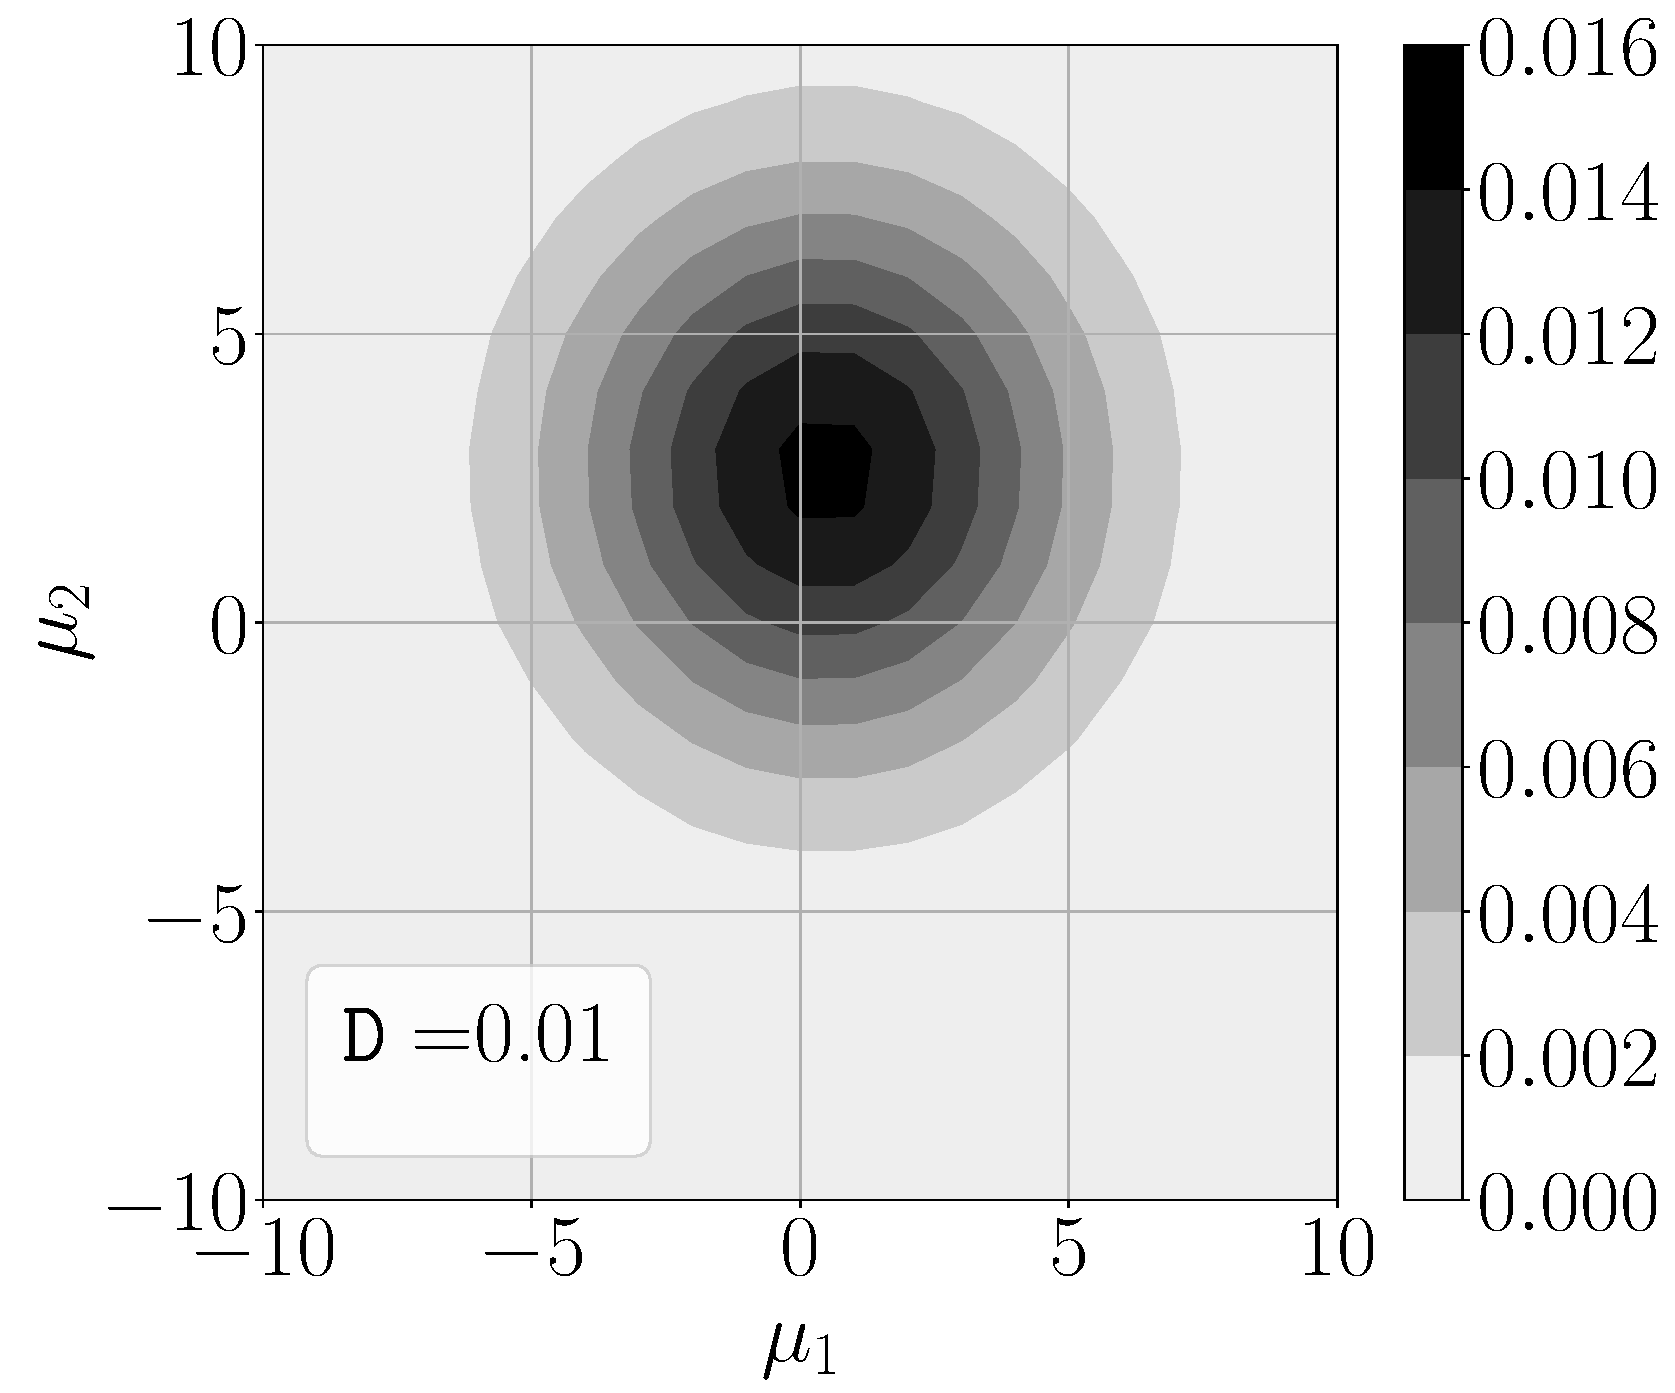
\includegraphics[width=\linewidth]{pics/double-homodyne/full.pdf}
\subcaption[]{}
        \end{minipage}
\hfill
        \begin{minipage}[c]{.45\linewidth}
 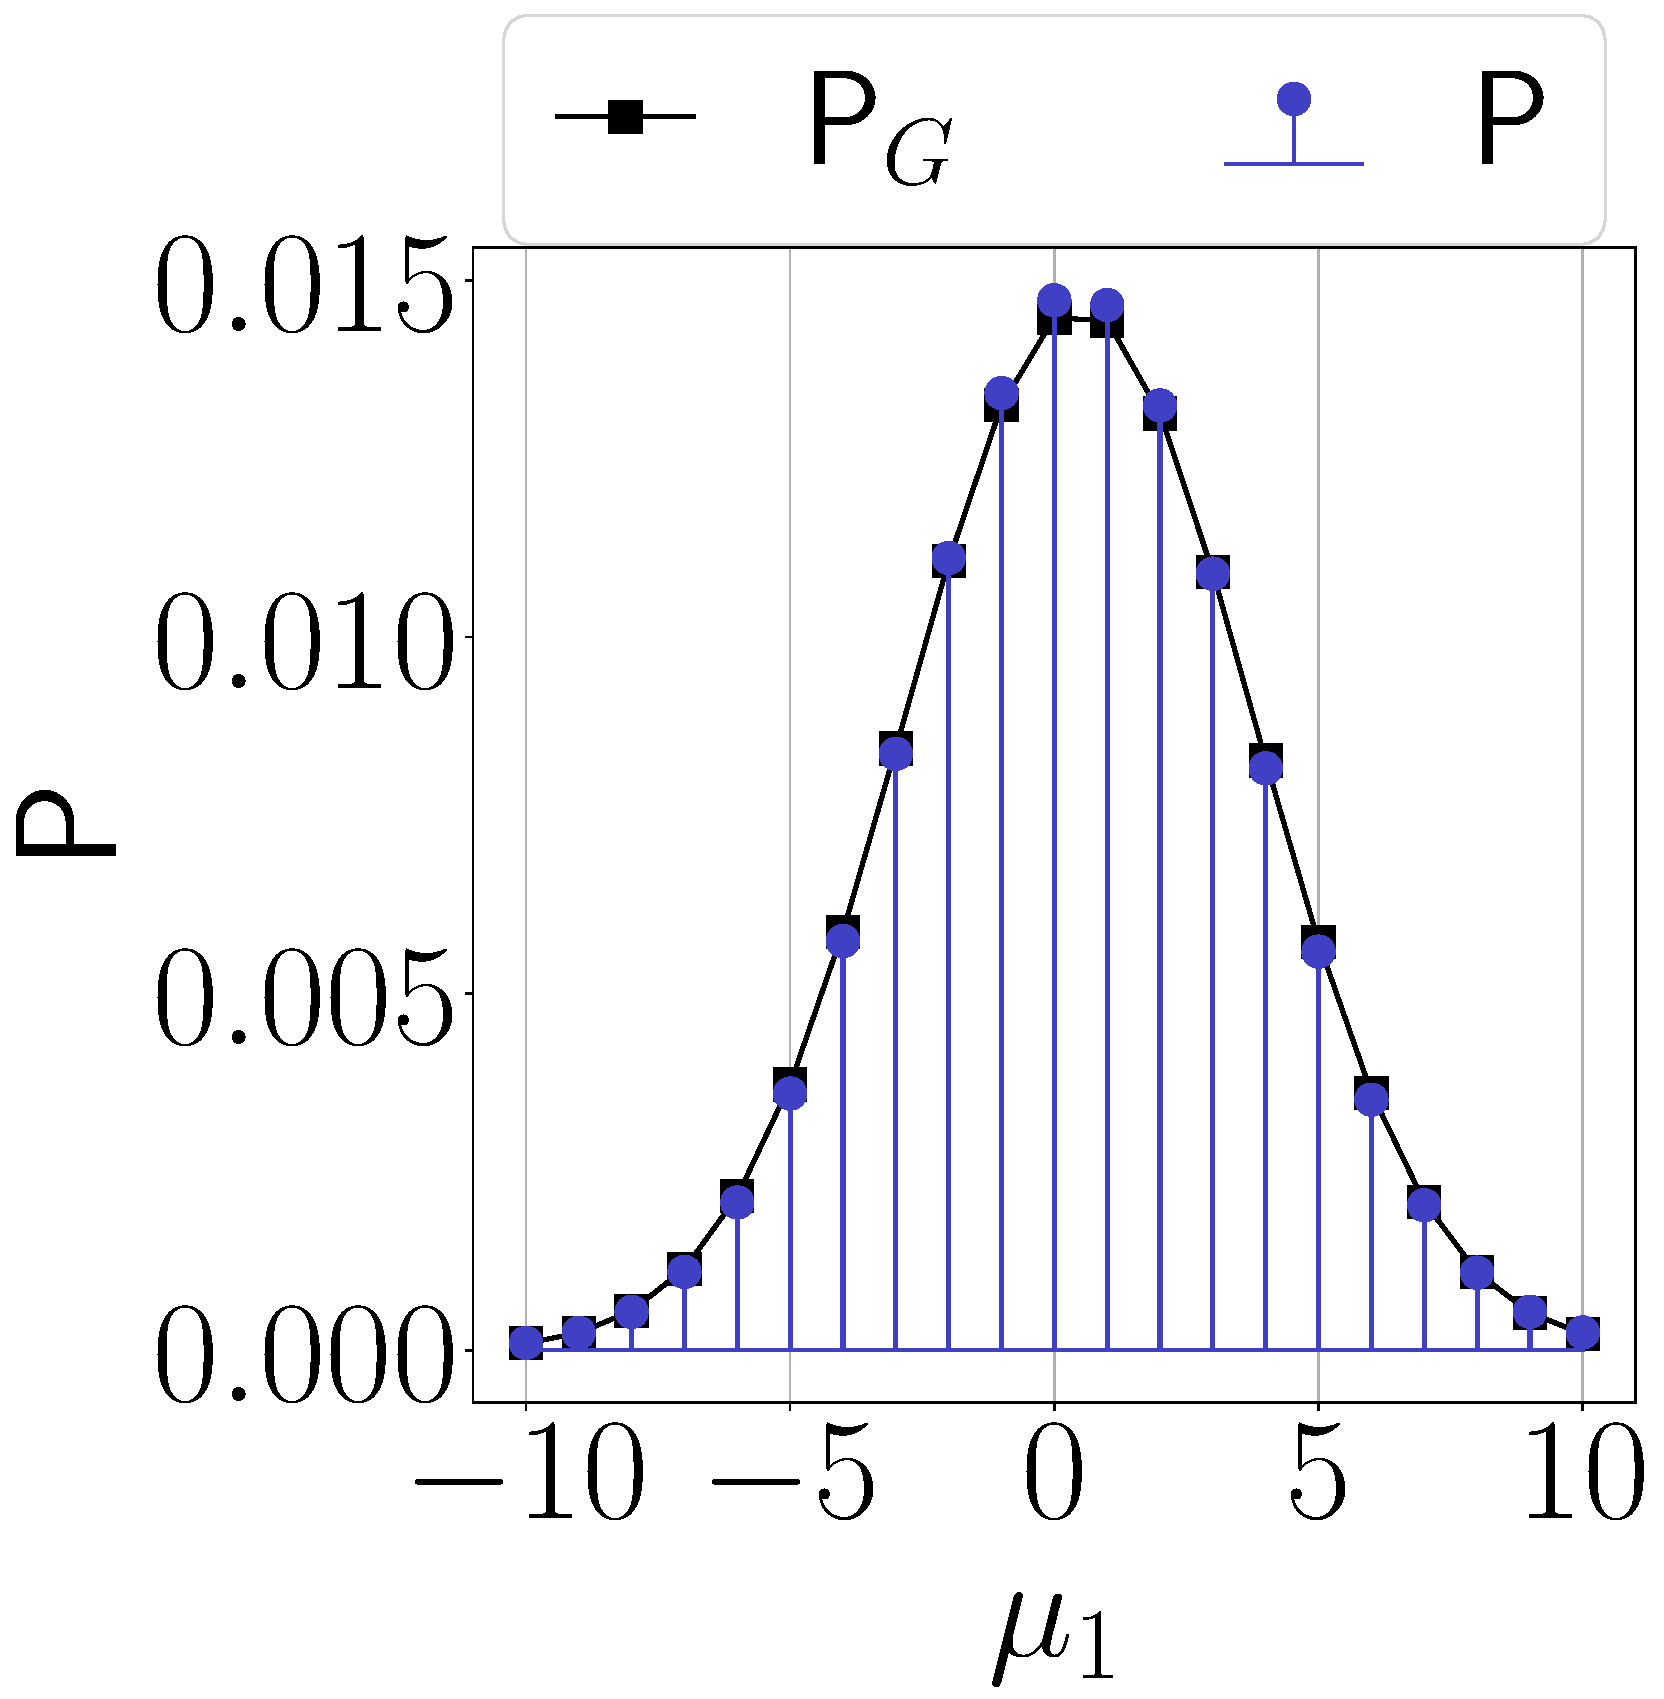
\includegraphics[width=\linewidth]{pics/double-homodyne/dm1.pdf}
\subcaption[]{}
\end{minipage}
\hfill
        \begin{minipage}[c]{.45\linewidth}
 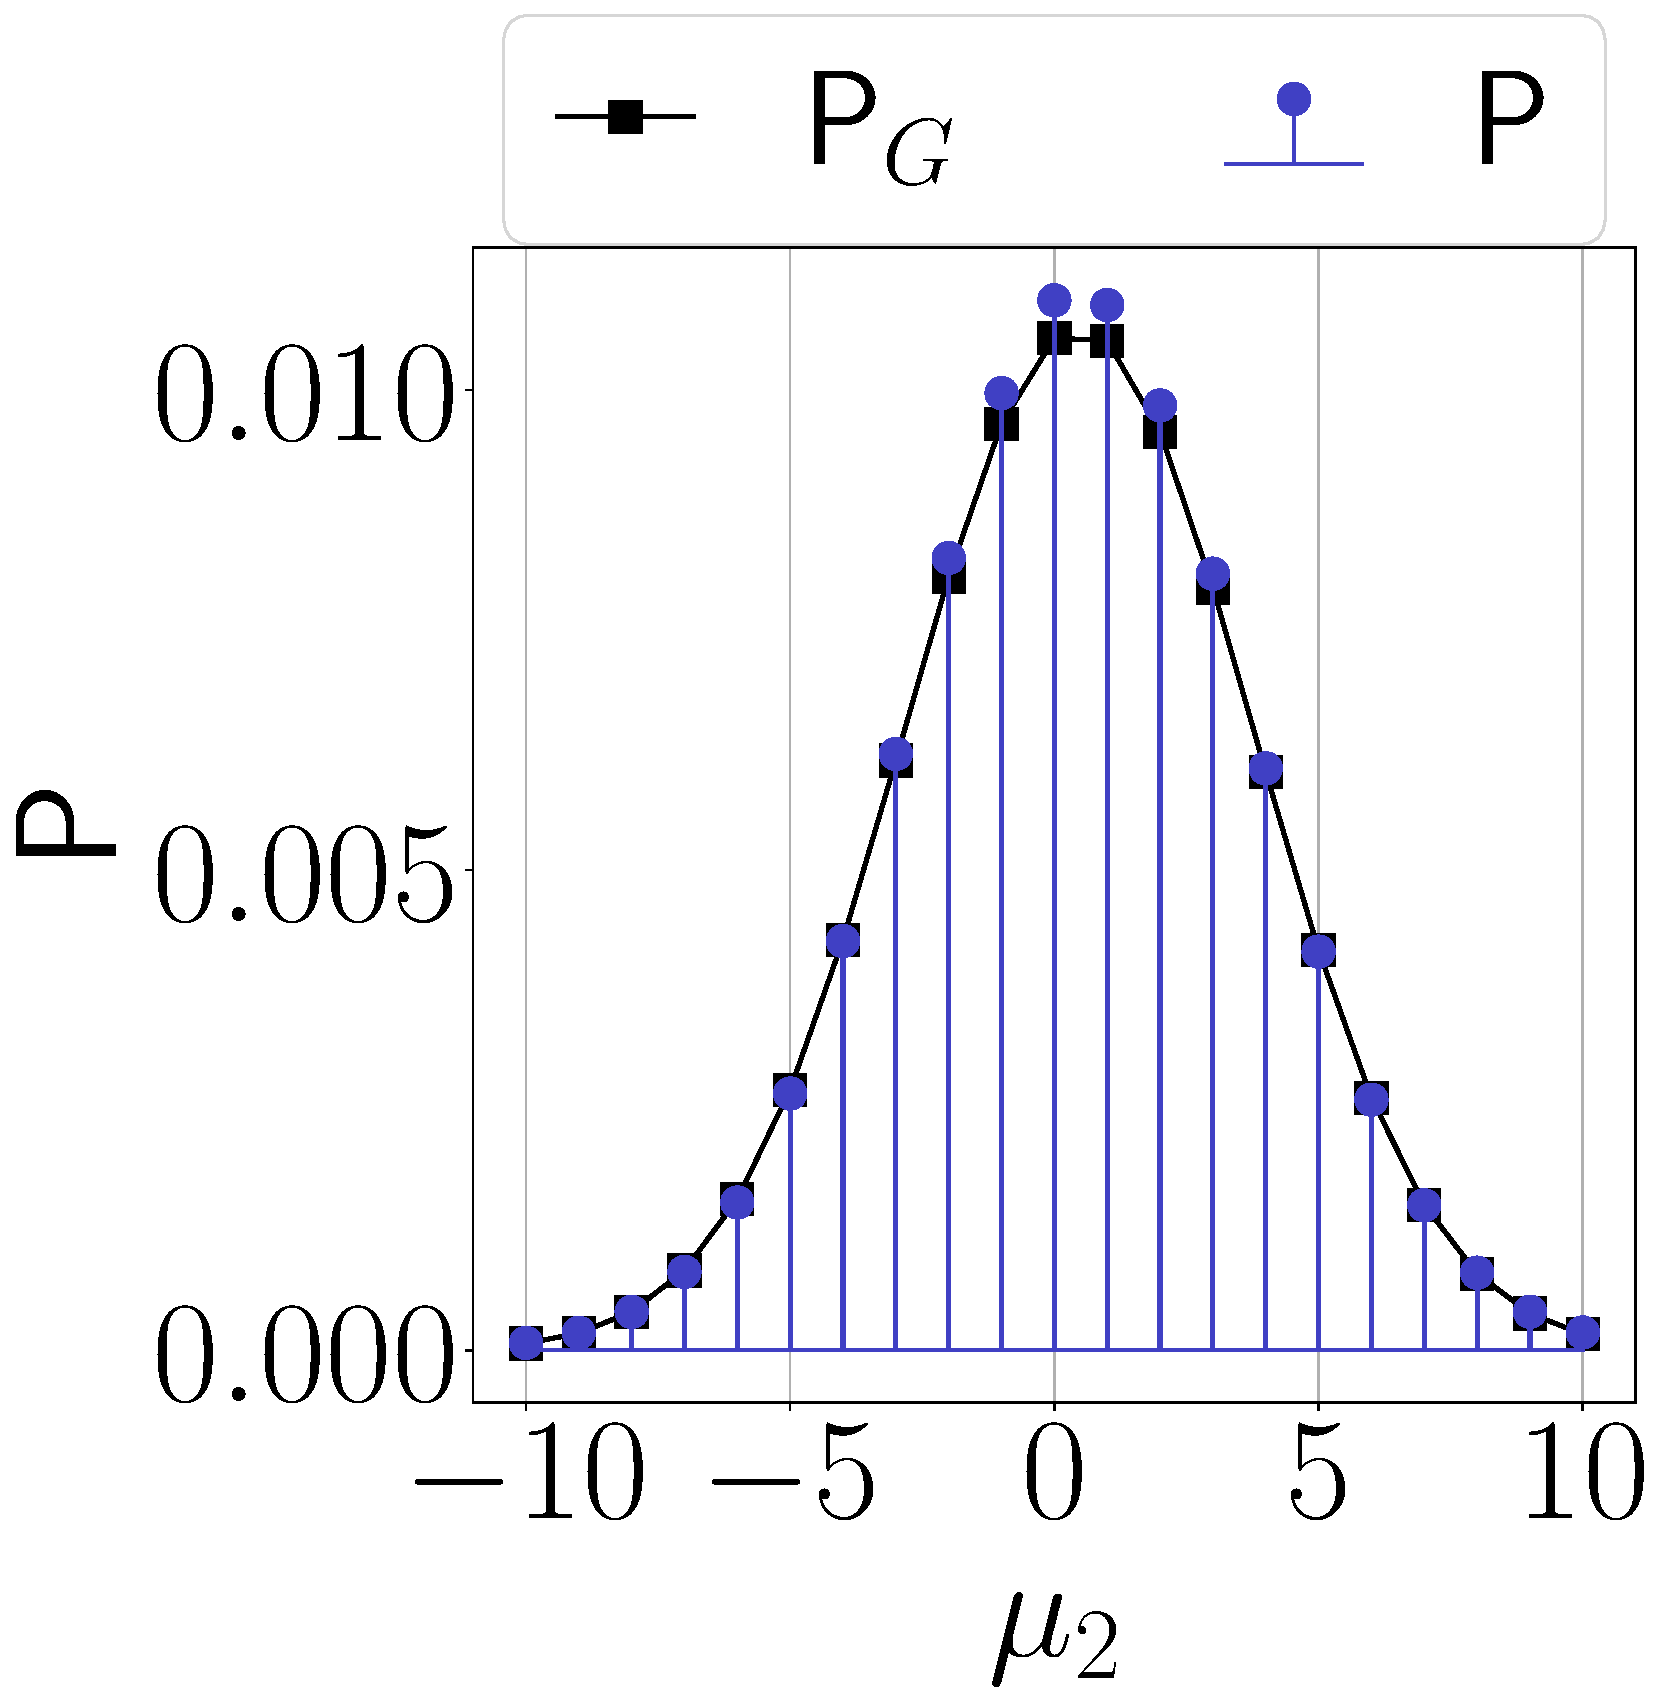
\includegraphics[width=\linewidth]{pics/double-homodyne/dm2.pdf}
\subcaption[]{}
\end{minipage}
    \caption{(a) -- 
     Numerically calculated exact statistical distribution of photon count difference in asymmetrical double homodyne scheme, given by  Eq.~\eqref{eq:accurate-dh}, and calculated distance between this distribution and approximate distribution, given by Eq.~\eqref{eq:Pgood-dh}; (b), (c) -- Projections of exact (blue) and approximate (black) statistical distributions of photon count difference, all calculated for parameters $\alpha=0.25+0.25i$, $\alpha_L=5$, $\eta_1=\eta_3=1$ and $\eta_2=\eta_4=0.75$.
    }\label{fig:dh-statistics}
\end{figure}
%\section{Experiment}\label{sec-experiment}
\section{Results and discussion}\label{sec-results}
We have derived the Gaussian approximation for the asymmetrical case of the homodyne scheme and used it to construct a well-defined POVM. This POVM is applicable across all parameter settings of the scheme. Our results both agree and extend the existing relations~\cite{braunstein1990homodyne}.

We evaluated the accuracy of our approximation {for all asymmetry parameters, namely relationship and absolute values of quantum detectors' efficiencies and transmission/reflection coefficieciets of the beamsplitter, as well as the dependance on signal and reference mode amplitudes}. Our findings indicate that the quality of the agreement between the exact and approximate solutions varies with the degree of asymmetry. By varying parameters of BS we may achieve the best approximation for given quantum efficiencies and vice versa. Results agree with other works on this subject, such as \cite{OLIVARES2020126354}. {We have found that Gaussian approximation is adequate even in edge cases of very weak LO amplitude or full transmission/reflection of BS.}

Developed formalism allows us to easily analyze various homodyne-based detection schemes. It can be extended to describe more complex measurement systems. We showcased this by analyzing the $8$-port double homodyne scheme. However, we encountered a problem with definition of Gaussian function, which needs further investigating. \hl{We presume that it is connected to usage of squeezed coherent states, see Ref.{~\cite{doi:10.1080/09500348714550131}}}

Additionally, we found that the {Skellam distribution approximation}, traditionally used for the strong Local Oscillator approximation, is not suitable for the asymmetrical case. 

%Comment on experimental data

\section{Conclusion}\label{sec-conclusion}
We developed a method of constructing the respective POVM of homodyne-based detection schemes. This method relies on approximating the exact statistics {of photon count difference} with Gaussian approximation. We applied this method to write POVM for homodyne and double homodyne schemes. For the double homodyne scheme, we have encountered a problem with our approach, {and our constructed POVM is not defined for all parameters of the scheme as expected}. This problem needs further investigating. Moreover, we have studied the applicability of Gaussian approximation in case of unequal non-unity quantum efficiency of photodetectors and unbalanced beam splitters. We have found that the usual approach of approximating the Skellam distribution using the asymptotic expansion of the modified Bessel function
of the first kind is not applicable in the asymmetrical case. {This is due to extremely poor quality of approximation and inability to construct the respective POVM with terms caused by asymmetry.}

\printbibliography
\clearpage
\appendix
\section{Skellam-based Gaussian approximation}%???????
\label{app:bessel}
In this section, we present another way of approximating Eq.~\eqref{eq:accurate}, which we duplicate here for convenience:
\begin{equation}
  P=e^{-\eta_1|\alpha_1|^2}e^{-\eta_2|\alpha_2|^2}
\left(\frac{\eta_1|\alpha_1|^2}{\eta_2|\alpha_2|^2}\right)^{\frac{\delta m}{2}}
I_{\delta m}\left(2\sqrt{\eta_1\eta_2|\alpha_1|^2|\alpha_2|^2}\right),\label{eq:Skellam}
\end{equation}
%where $I_k(z)$ is the modified Bessel function of the first kind, and the transformed amplitudes $|\alpha_{1,2}|$ are given by Eq.~\eqref{eq:amplitudes}.


In the strong LO approximation, where $|\alpha_L|\gg|\alpha|$, the Bessel function $I_k(z)$ can be approximated using its asymptotic expression for large $|z|$ and $k$, with finite $\sqrt{\left|\frac{k^2}{z}\right|}$ (see Ref.~\cite{doi:10.1080/09500349808231235,freyberger1993photon}),
\begin{equation}
    I_k(z)\approx\frac{1}{\sqrt{2\pi z}}\exp\left[z-\frac{k^2}{z}\right]. \label{eq:hole}
\end{equation}
Assuming $C\not\to0$ and $S\not\to0$, (which avoids contradictions in the strong LO approximation as per Eq.~\eqref{eq:amplitudes}) and that $(CS)^{-1}$ remains finite, we can approximate the terms in the Skellam distribution as follows:
\begin{equation}
    |\alpha_1||\alpha_2|
    \approx
    CS|\alpha_L|^2\left[1+\frac{C^2-S^2}{(CS)^2}\frac{2CS\Re\alpha\alpha_L^*}{|\alpha_L|^2}\right]^{\frac{1}{2}}
    \approx
    CS|\alpha_L|^2+\left(C^2-S^2\right){\Re\alpha\alpha_L^*},
\end{equation}
\begin{multline}
    \exp\left[
    2\sqrt{\eta_1\eta_2}|\alpha_1||\alpha_2|-\eta_1|\alpha_1|^2-\eta_2|\alpha_2|^2
    \right]\approx
\\
    \approx\exp\left[-\left(|\alpha_L|(S\sqrt{\eta_1}-C\sqrt{\eta_2})+\frac{CS\Re\alpha\alpha_L^*}{|\alpha_L|}\left\{S\sqrt{\eta_1}+C\sqrt{\eta_2}\right\}\right)^2\right],
\end{multline}
\begin{equation}
        \left(\frac{{\eta_1}|\alpha_1|^2}{{\eta_2}|\alpha_2|^2}\right)^{\frac{\delta m}{2}}\approx
    \exp\left[\frac{\delta m}{2}\left(
    \ln\frac{\eta_1S^2}{\eta_2C^2}+\frac{2\Re\alpha\alpha_L^*}{CS|\alpha_L|^2}\right)
    \right],
    \label{eq:hole2}
\end{equation}
then we obtain the following approximation of Eq.~\eqref{eq:Skellam}:
\begin{multline}
        P_B=
    \frac{1}{\sqrt{4\pi\sqrt{\eta_1\eta_2}\left(CS|\alpha_L|^2+(C^2-S^2){\Re\alpha\alpha_L^*}\right)}}
    \times\\\times\exp\biggl[
    -\frac{\delta m^2}{4\sqrt{\eta_1\eta_2}\left(CS|\alpha_L|^2+\left(C^2-S^2\right){\Re\alpha\alpha_L^*}\right)}-\\-\left(
|\alpha_L|(S\sqrt{\eta_1}-C\sqrt{\eta_2})+\frac{CS\Re\alpha\alpha_L^*}{|\alpha_L|}\left\{
S\sqrt{\eta_1}+C\sqrt{\eta_2}
\right\}
\right)^2
    +\\+
    \frac{\delta m}{2}\left(
    \ln\frac{\eta_1S^2}{\eta_2C^2}+\frac{4CS\Re\alpha\alpha_L^*}{|\alpha_L|^2}\right)
    \biggr],
\end{multline}
which simplifies to:
\begin{multline}
    P_B=\frac{1}{\sqrt{4\pi\sqrt{\eta_1\eta_2}\left(CS|\alpha_L|^2+(C^2-S^2)\Re\alpha\alpha_L^*\right)}}
    \times\\\times\exp\biggl[-\frac{1}{2}\frac{\sqrt{\eta_1\eta_2}}{2CS}
    \biggl(\frac{\delta m}{{\sqrt{\eta_1\eta_2}|\alpha_L|}}-
    CS|\alpha_L|\ln\frac{\eta_1S^2}{\eta_2C^2}-\langle\hat{x}_\phi\rangle
    \biggr)^2\biggr],\label{eq:Pbad}
\end{multline}
to this we will refer as "Skellam-based Gaussian approximation".
Note that Eq.~\eqref{eq:Pgood} and Eq.~\eqref{eq:Pbad} are equivalent for the symmetric case. However, expressing $P_B$ in the form of Eq.~\eqref{eq:theform} and using Eq.~\eqref{eq:conv} gives
\begin{equation}
    2\frac{2CS}{\sqrt{\eta_1\eta_2}}=\sigma+2.
\end{equation}
This implies that $\sigma$ can be negative for certain combinations of $\eta_{1,2}$ and $\theta$ (e.g $\eta_1+\eta_2<2, \theta\neq{\pi}/{4}$), which contradicts the form given in Eq.~\eqref{eq:theform}. Therefore, Eq.~\eqref{eq:Pbad} does not fully describe the asymmetrical case, and this is a direct consequence of Eq.~\eqref{eq:hole}. Numerical results (see Fig.~\ref{fig:PB_PG}) also indicate that $P_B$ is less accurate than $P_G$ for approximating Eq.~\eqref{eq:accurate} in cases of higher asymmetry. Moreover, we can pinpoint the cause of worse performance to terms given by Eq.~\eqref{eq:hole} and Eq.~\eqref{eq:hole2}. We draw this conclusion from the difference in shifting of exact and approximate formulae, which are described by these terms. To further prove this, we will calculate the relation:
\begin{equation}
    \frac{I_{\delta m}(z)
    }{\frac{1}{\sqrt{2\pi z}}\exp\left[z-\frac{k^2}{z}\right]}
    \frac{\left(\frac{{\eta_1}|\alpha_1|^2}{{\eta_2}|\alpha_2|^2}\right)^{\frac{\delta m}{2}}}{\exp\left[\frac{\delta m}{2}\left(
    \ln\frac{\eta_1S^2}{\eta_2C^2}+\frac{2\Re\alpha\alpha_L^*}{CS|\alpha_L|^2}\right)
    \right]}
    ,\label{eq:relation}
\end{equation}
where $z\equiv2\sqrt{\eta_1\eta_2|\alpha_1|^2|\alpha_2|^2}$, as a function of $\theta$. Results are presented in Fig.~\ref{fig:relation}, from which we may see that at high asymmetry these approximations do not hold.
\begin{figure}
    \centering
    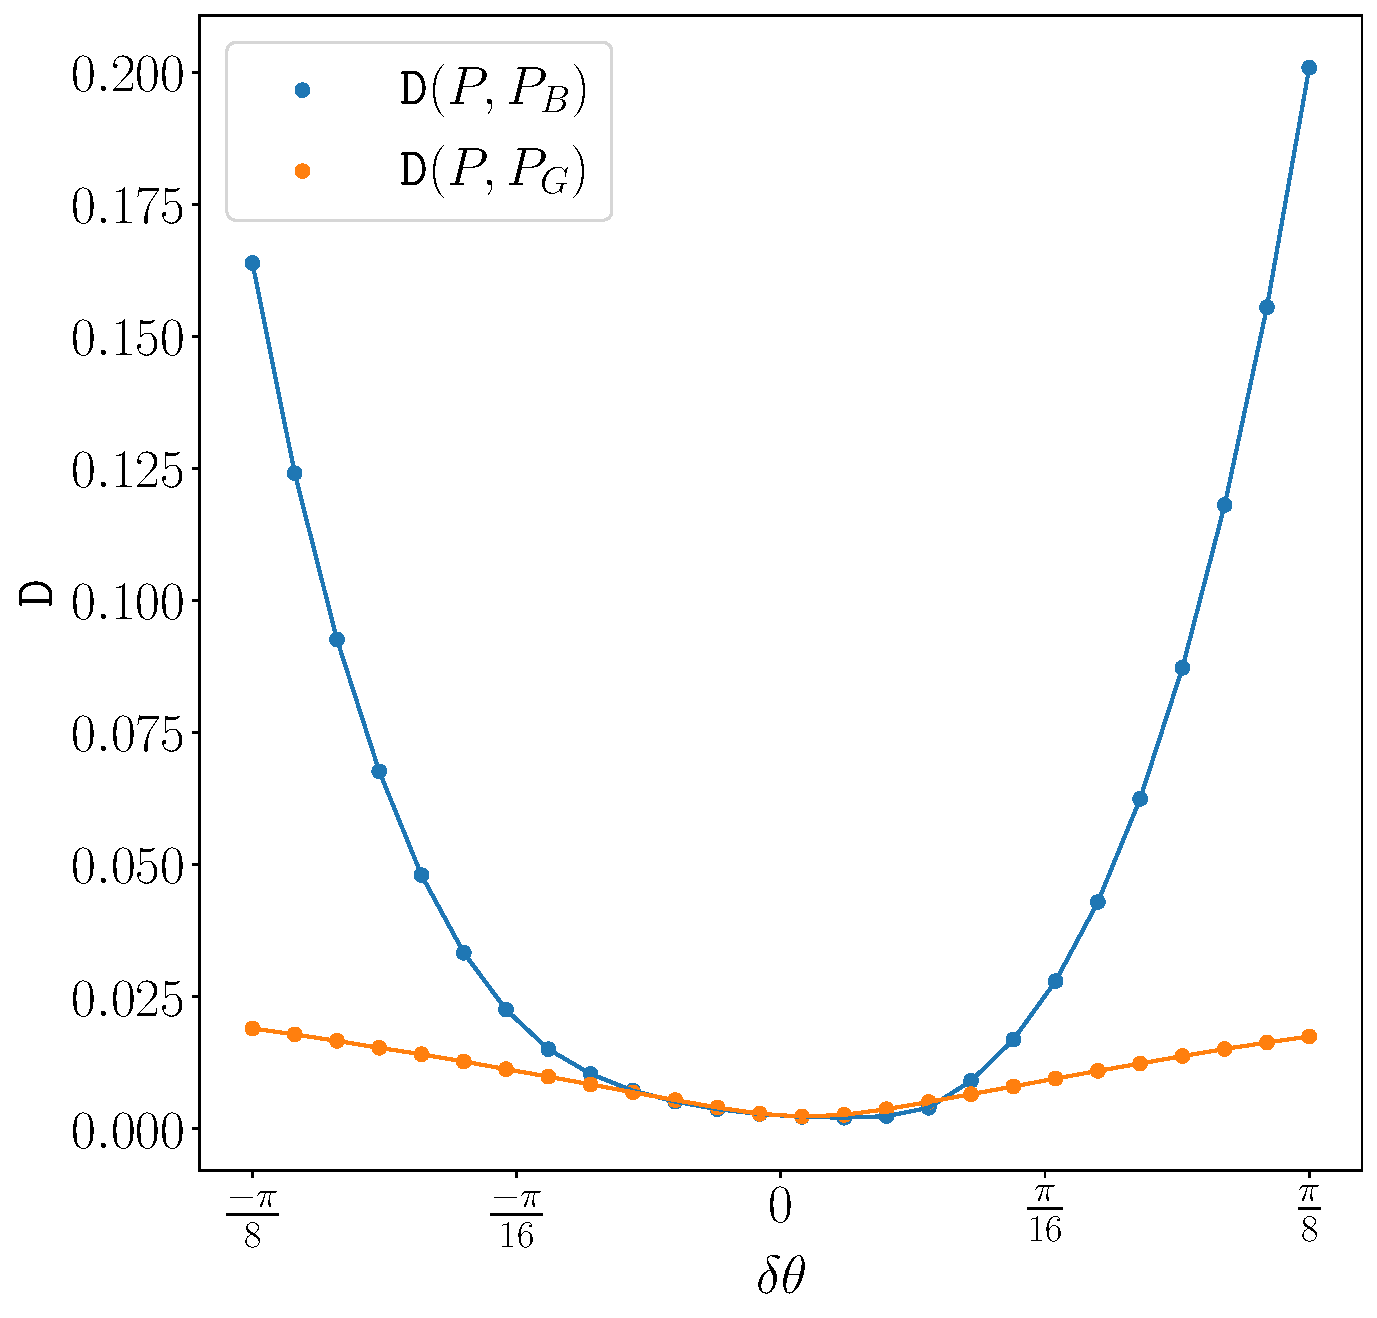
\includegraphics[width=\linewidth]{pics/appendix/theta.pdf}
    \caption{Distance between the exact statistical distribution and Gaussian (orange) and Skellam-based Gaussian (blue) approximations as a function of $\delta\theta$ with $\eta_1=\eta_2=1$. Note the significant difference (in first decimal places) between the curves, which means that $P_B$ becomes incorrect for higher asymmetry}
    \label{fig:PB_PG}
\end{figure}

\begin{figure}
    \centering
    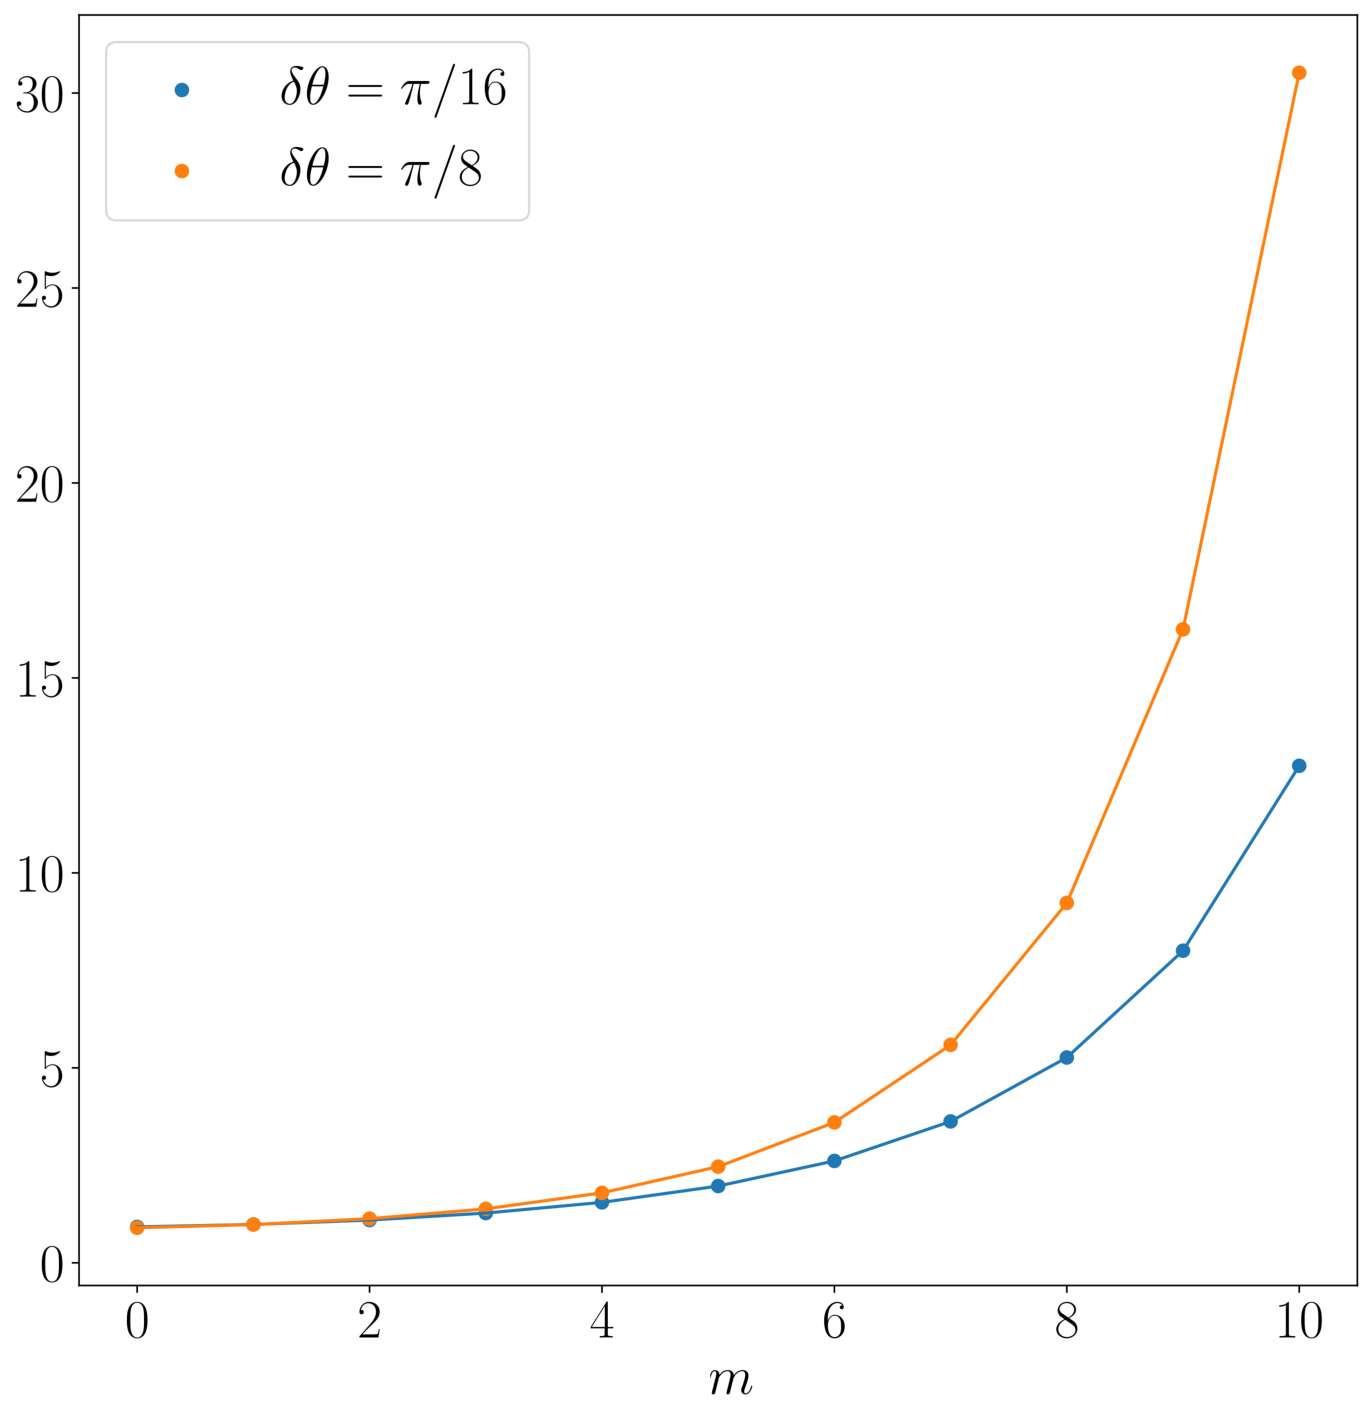
\includegraphics[width=0.75\linewidth]{pics/appendix/relation.pdf}
    \caption{Relation represented by Eq.~\eqref{eq:relation}, plotted against $\delta m$, with parameters $\eta_1=\eta_2=1, |\alpha|=0.1$ and $|\alpha_L|=5$, for various $\delta\theta$. Significant deviation from unity represents incorrectness of approximations Eq.~\eqref{eq:hole} and Eq.~\eqref{eq:hole2}.}
    \label{fig:relation}
\end{figure}
\end{document}
